\clearpage
\section{لوحات المعلومات}
\label{sec:builder-feature-dashboards}

لوحة المعلومات صفحة أرقام ورسوم بيانية تلخّص العمل، مثل عدد الطلبات المفتوحة أو المتأخرة. وتبدأ كل لوحة من صفحة «لوحات المعلومات»، وفيها تُنشئ اللوحات وترتّبها في مجلدات وتحدد من يصل إلى كل منها. أما بناء محتوى اللوحة فيجري في منشئ اللوحة الذي تشرحه الصفحات التالية.

\textbf{المسار ومن يستخدمه:} «ادوات البناء» ← «الأساسية» ← «لوحات المعلومات». يظهر زر «إنشاء لوحة معلومات» لمن يملك صلاحية إنشاء اللوحات، ويرى كل مستخدم البطاقات التي يملك صلاحية فتحها.

\begin{rcnote}[مثال: شركة الأفق]
ينشئ مسؤول النظام مجلداً باسم «خدمات الفروع»، ثم ينشئ داخله لوحة «متابعة الزيارات» ويمنح دور سارة الخطيب الوصول إليها. وتبدأ اللوحة من ①، ويبدأ المجلد من ②.
\end{rcnote}

\begin{figure}[H]
\centering
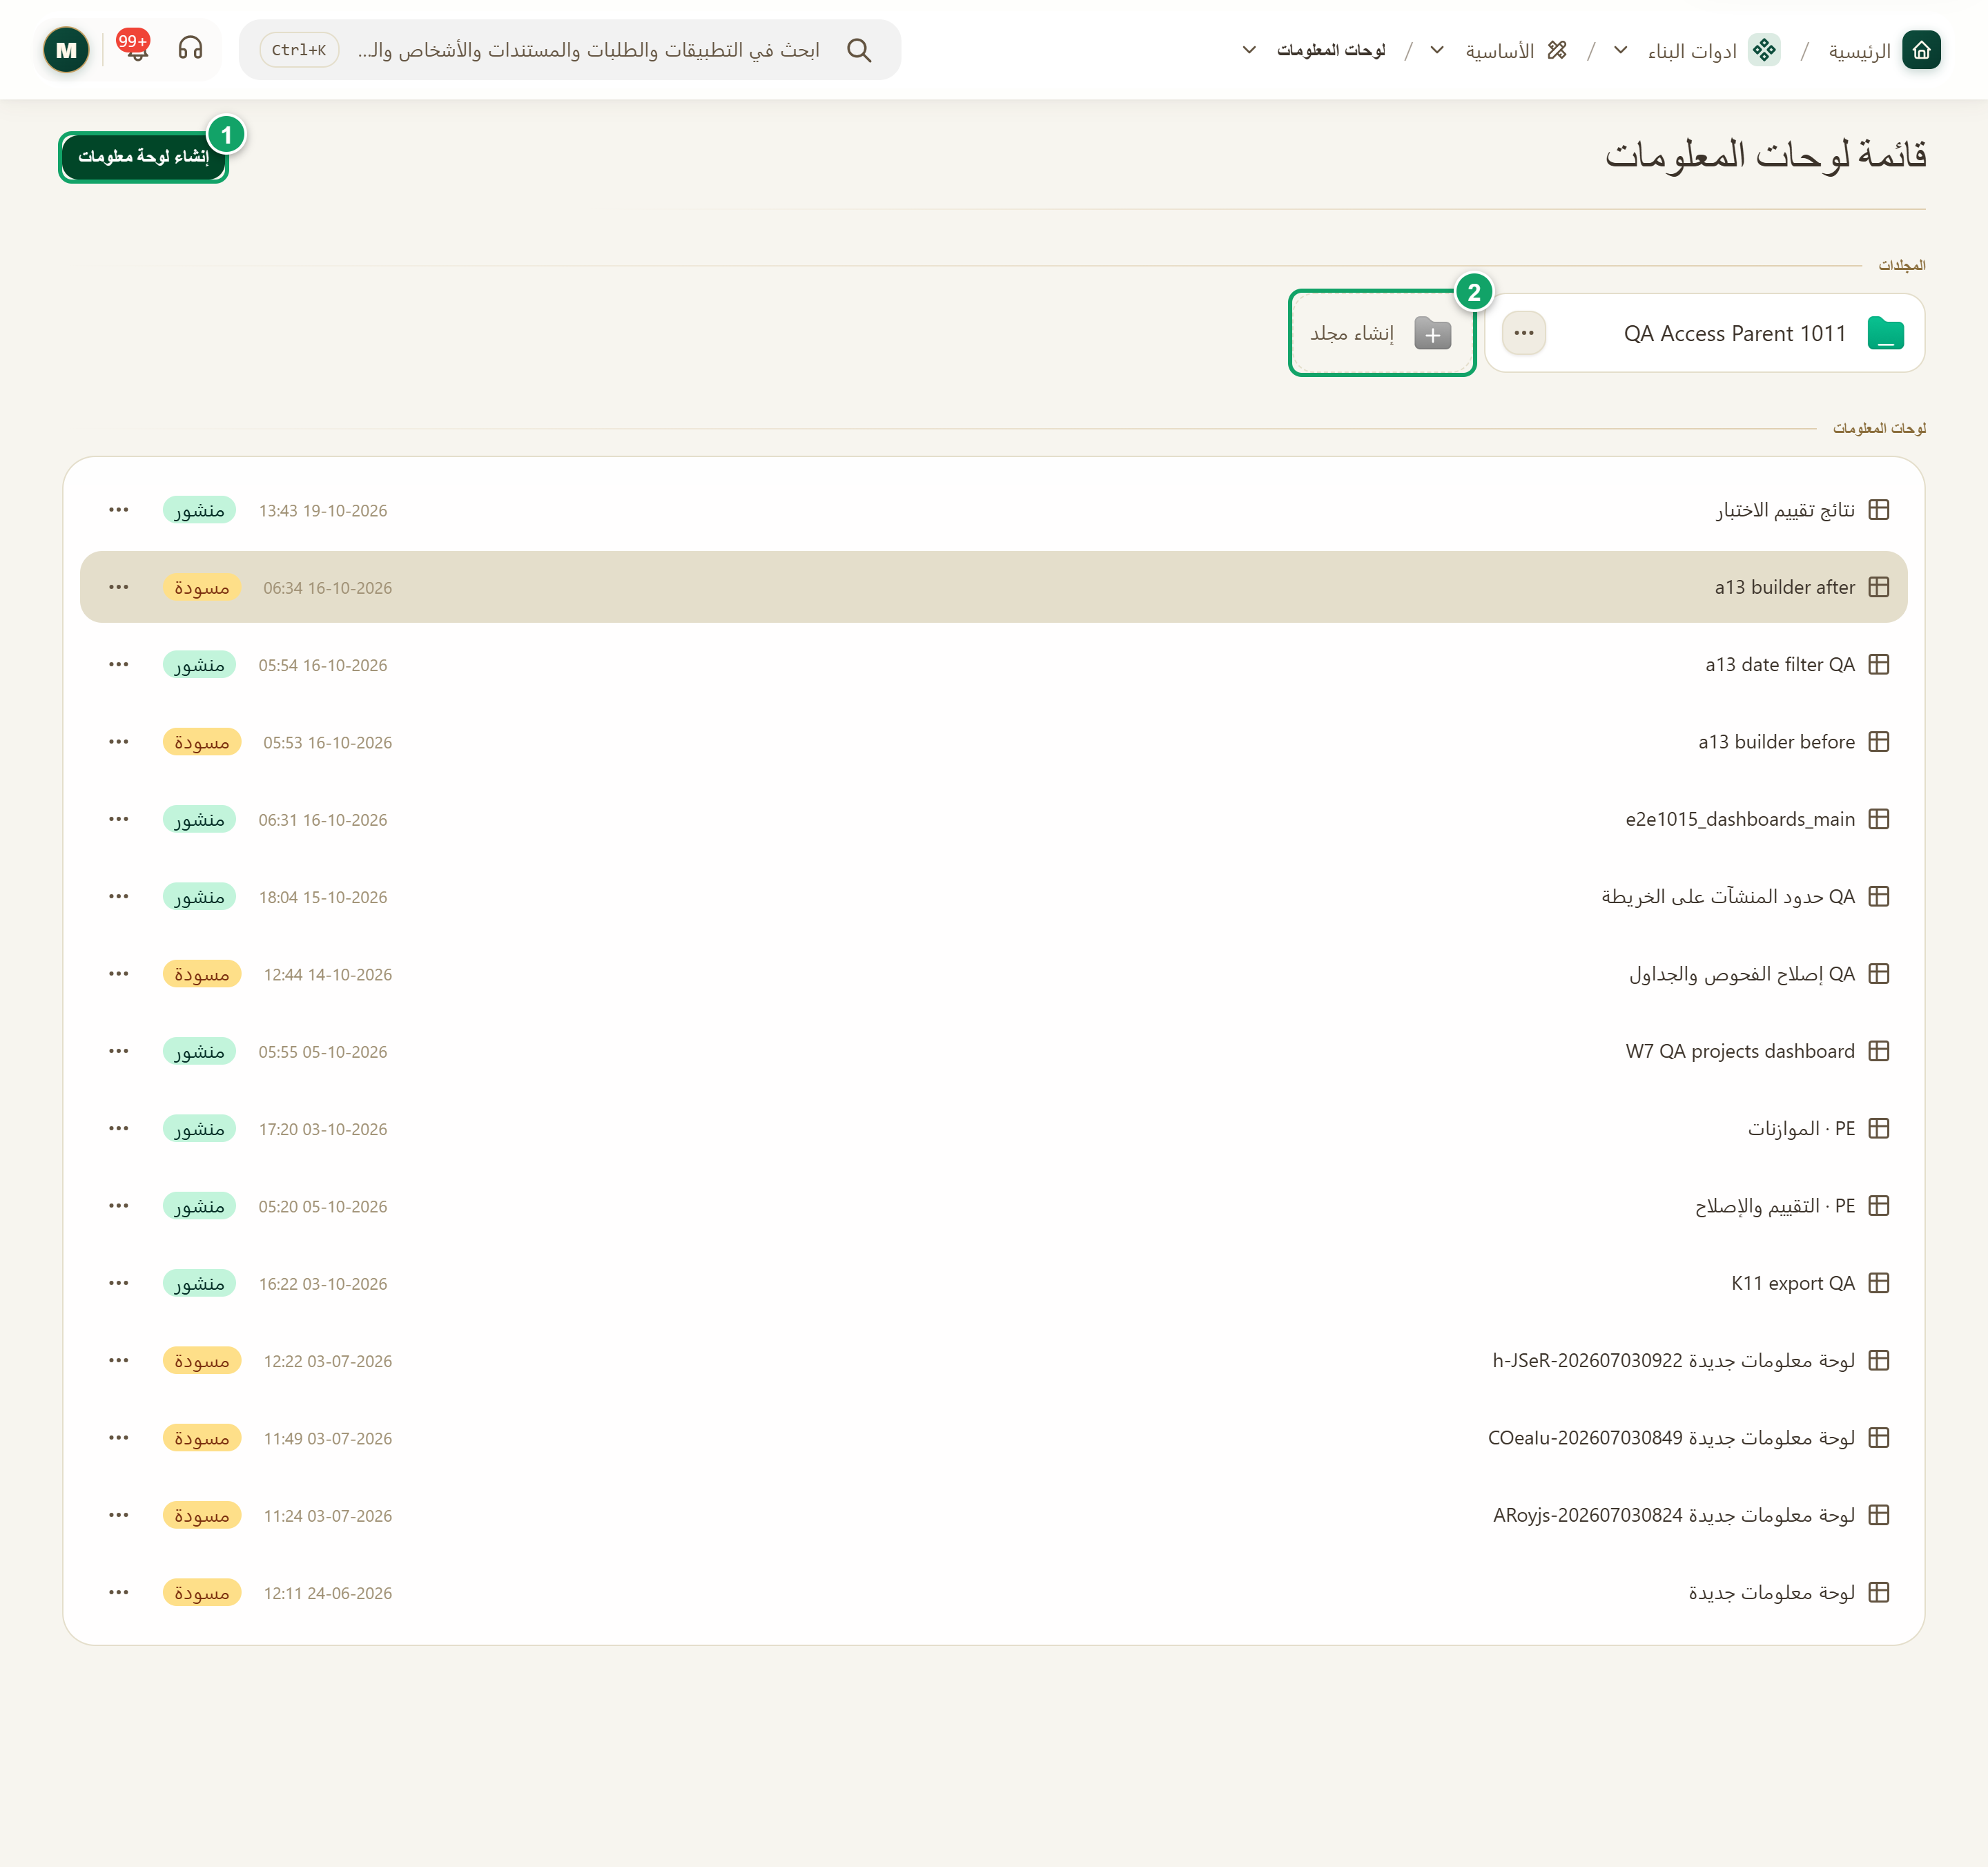
\includegraphics[width=0.95\linewidth,height=0.72\textheight,keepaspectratio]{figures/screens/ch06-dashboards-ar.png}
\caption{صفحة «لوحات المعلومات»}
\label{fig:builder-dashboards-screen}
\shotnote{تعرض الصفحة المجلدات ولوحات المعلومات مع حالتها، وهي هنا لوحات اختبار. ① «إنشاء لوحة معلومات»: تبدأ لوحة جديدة. ② «إنشاء مجلد»: ينظّم اللوحات في مجلدات.}
\end{figure}


\begin{table}[H]
\centering
\caption{ما الذي تجده في القائمة؟}
\label{tab:builder-dashboards-data}
\begin{tabularx}{\linewidth}{R{3.6cm} Y}
\rcHeaderRow
\thh{الجزء} & \thh{المحتوى والإجراء}\\
بطاقة اللوحة & تعرض اسم اللوحة وآخر تعديل عليها وحالتها: «مسودة» إذا لم تُنشر بعد، أو «منشور». وتفتح قائمتها الإجراءات «عرض» و«تعديل» و«إدارة الصلاحيات» و«حذف» بحسب صلاحياتك.\\
«إنشاء لوحة معلومات» & تطلب «اسم لوحة المعلومات» ووصفاً لا يقل عن اثني عشر حرفاً وكلمتين، ثم تفتح اللوحة الجديدة في المنشئ. وتُنشأ اللوحة داخل المجلد المفتوح.\\
المجلدات & «إنشاء مجلد» ينشئ مجلداً يضم لوحات ومجلدات فرعية. وتنقل اللوحة إليه بسحب بطاقتها وإفلاتها فوقه، وتُنقل محتويات المجلد إلى خارجه عند حذفه.\\
الوصول & يحدد «إدارة الوصول» الأدوار والأشخاص الذين يفتحون اللوحة. وتحصل اللوحة أيضاً على الوصول الممنوح لمجلدها، فإزالة شخص من اللوحة لا تزيل وصوله من المجلد.\\
\end{tabularx}
\end{table}

\begin{figure}[H]
\centering
\begin{tikzpicture}[node distance=0.5cm]
\node[stepBox] (a) {\RL{إنشاء مجلد عند الحاجة}};
\node[stepBox,below=of a] (b) {\RL{إنشاء لوحة معلومات داخله}};
\node[stepBox,below=of b] (c) {\RL{البناء والنشر في المنشئ}};
\node[stepBox,below=of c] (d) {\RL{منح الوصول للأدوار}};
\draw[flowsTo] (a) -- (b);
\draw[flowsTo] (b) -- (c);
\draw[flowsTo] (c) -- (d);
\end{tikzpicture}
\rclegend
\caption{من القائمة إلى لوحة يصل إليها الفريق}
\label{fig:builder-dashboards-flow}
\shotnote{يبيّن المخطط أن مكان اللوحة يُحدَّد قبل إنشائها، لأنها تُنشأ داخل المجلد المفتوح وترث الوصول الممنوح له. ويأتي منح الوصول بعد النشر، لأن من يفتح لوحة غير منشورة يرى رسالة تفيد بأنها لم تُنشر بعد.}
\end{figure}

\subsection{خطوات العمل والتحقق}
\begin{enumerate}
\item افتح «لوحات المعلومات»، واضغط «إنشاء مجلد» إذا أردت تجميع لوحات قسم واحد، ثم افتح المجلد.
\item اضغط «إنشاء لوحة معلومات»، واكتب «اسم لوحة المعلومات» ووصفاً يشرح ما تتابعه اللوحة، ثم اضغط «إنشاء».
\item ابنِ اللوحة وانشرها كما في الصفحات التالية، ثم عُد إلى القائمة وتأكد أن حالتها «منشور».
\item اختر «إدارة الصلاحيات» من قائمة البطاقة، وأضف الأدوار التي يجب أن تراها.
\end{enumerate}

\textbf{تحقق ومعالجة المشكلة:} يجب أن تظهر البطاقة في المجلد الصحيح بحالة «منشور»، وأن يفتحها المستخدم المقصود. فإذا ظهرت رسالة «صِف في 12 حرفاً وكلمتين على الأقل»، فأطل الوصف. وإذا بقي شخص يرى اللوحة بعد إزالته، فراجع الوصول الممنوح على مجلدها.

\clearpage
\section{منشئ اللوحة: الأقسام والعناصر}
\label{sec:builder-feature-dashboards-builder}

منشئ اللوحة هو المكان الذي تبني فيه محتوى اللوحة. وتتكون اللوحة من أقسام متتالية، لكل قسم عنوان ووصف وشبكة تضع فيها العناصر، والعنصر هو رقم أو رسم بياني أو جدول أو غير ذلك. وتُحفظ تعديلاتك مسودةً بزر «حفظ»، ولا يراها المشاهدون حتى تنشرها.

\textbf{المسار ومن يستخدمه:} «لوحات المعلومات» ← قائمة بطاقة اللوحة ← «تعديل». يستخدمه من يملك صلاحية تعديل اللوحة، ويُفتح تلقائياً بعد إنشاء لوحة جديدة.

\begin{rcnote}[مثال: شركة الأفق]
يضيف مسؤول النظام إلى لوحة «متابعة الزيارات» قسماً بعنوان «حالة الطلبات» فيه رقم للطلبات المنتظرة ورسم دائري للطلبات حسب الحالة، ثم قسماً ثانياً بعنوان «المواعيد» فيه تقويم الزيارات.
\end{rcnote}

\begin{figure}[H]
\centering
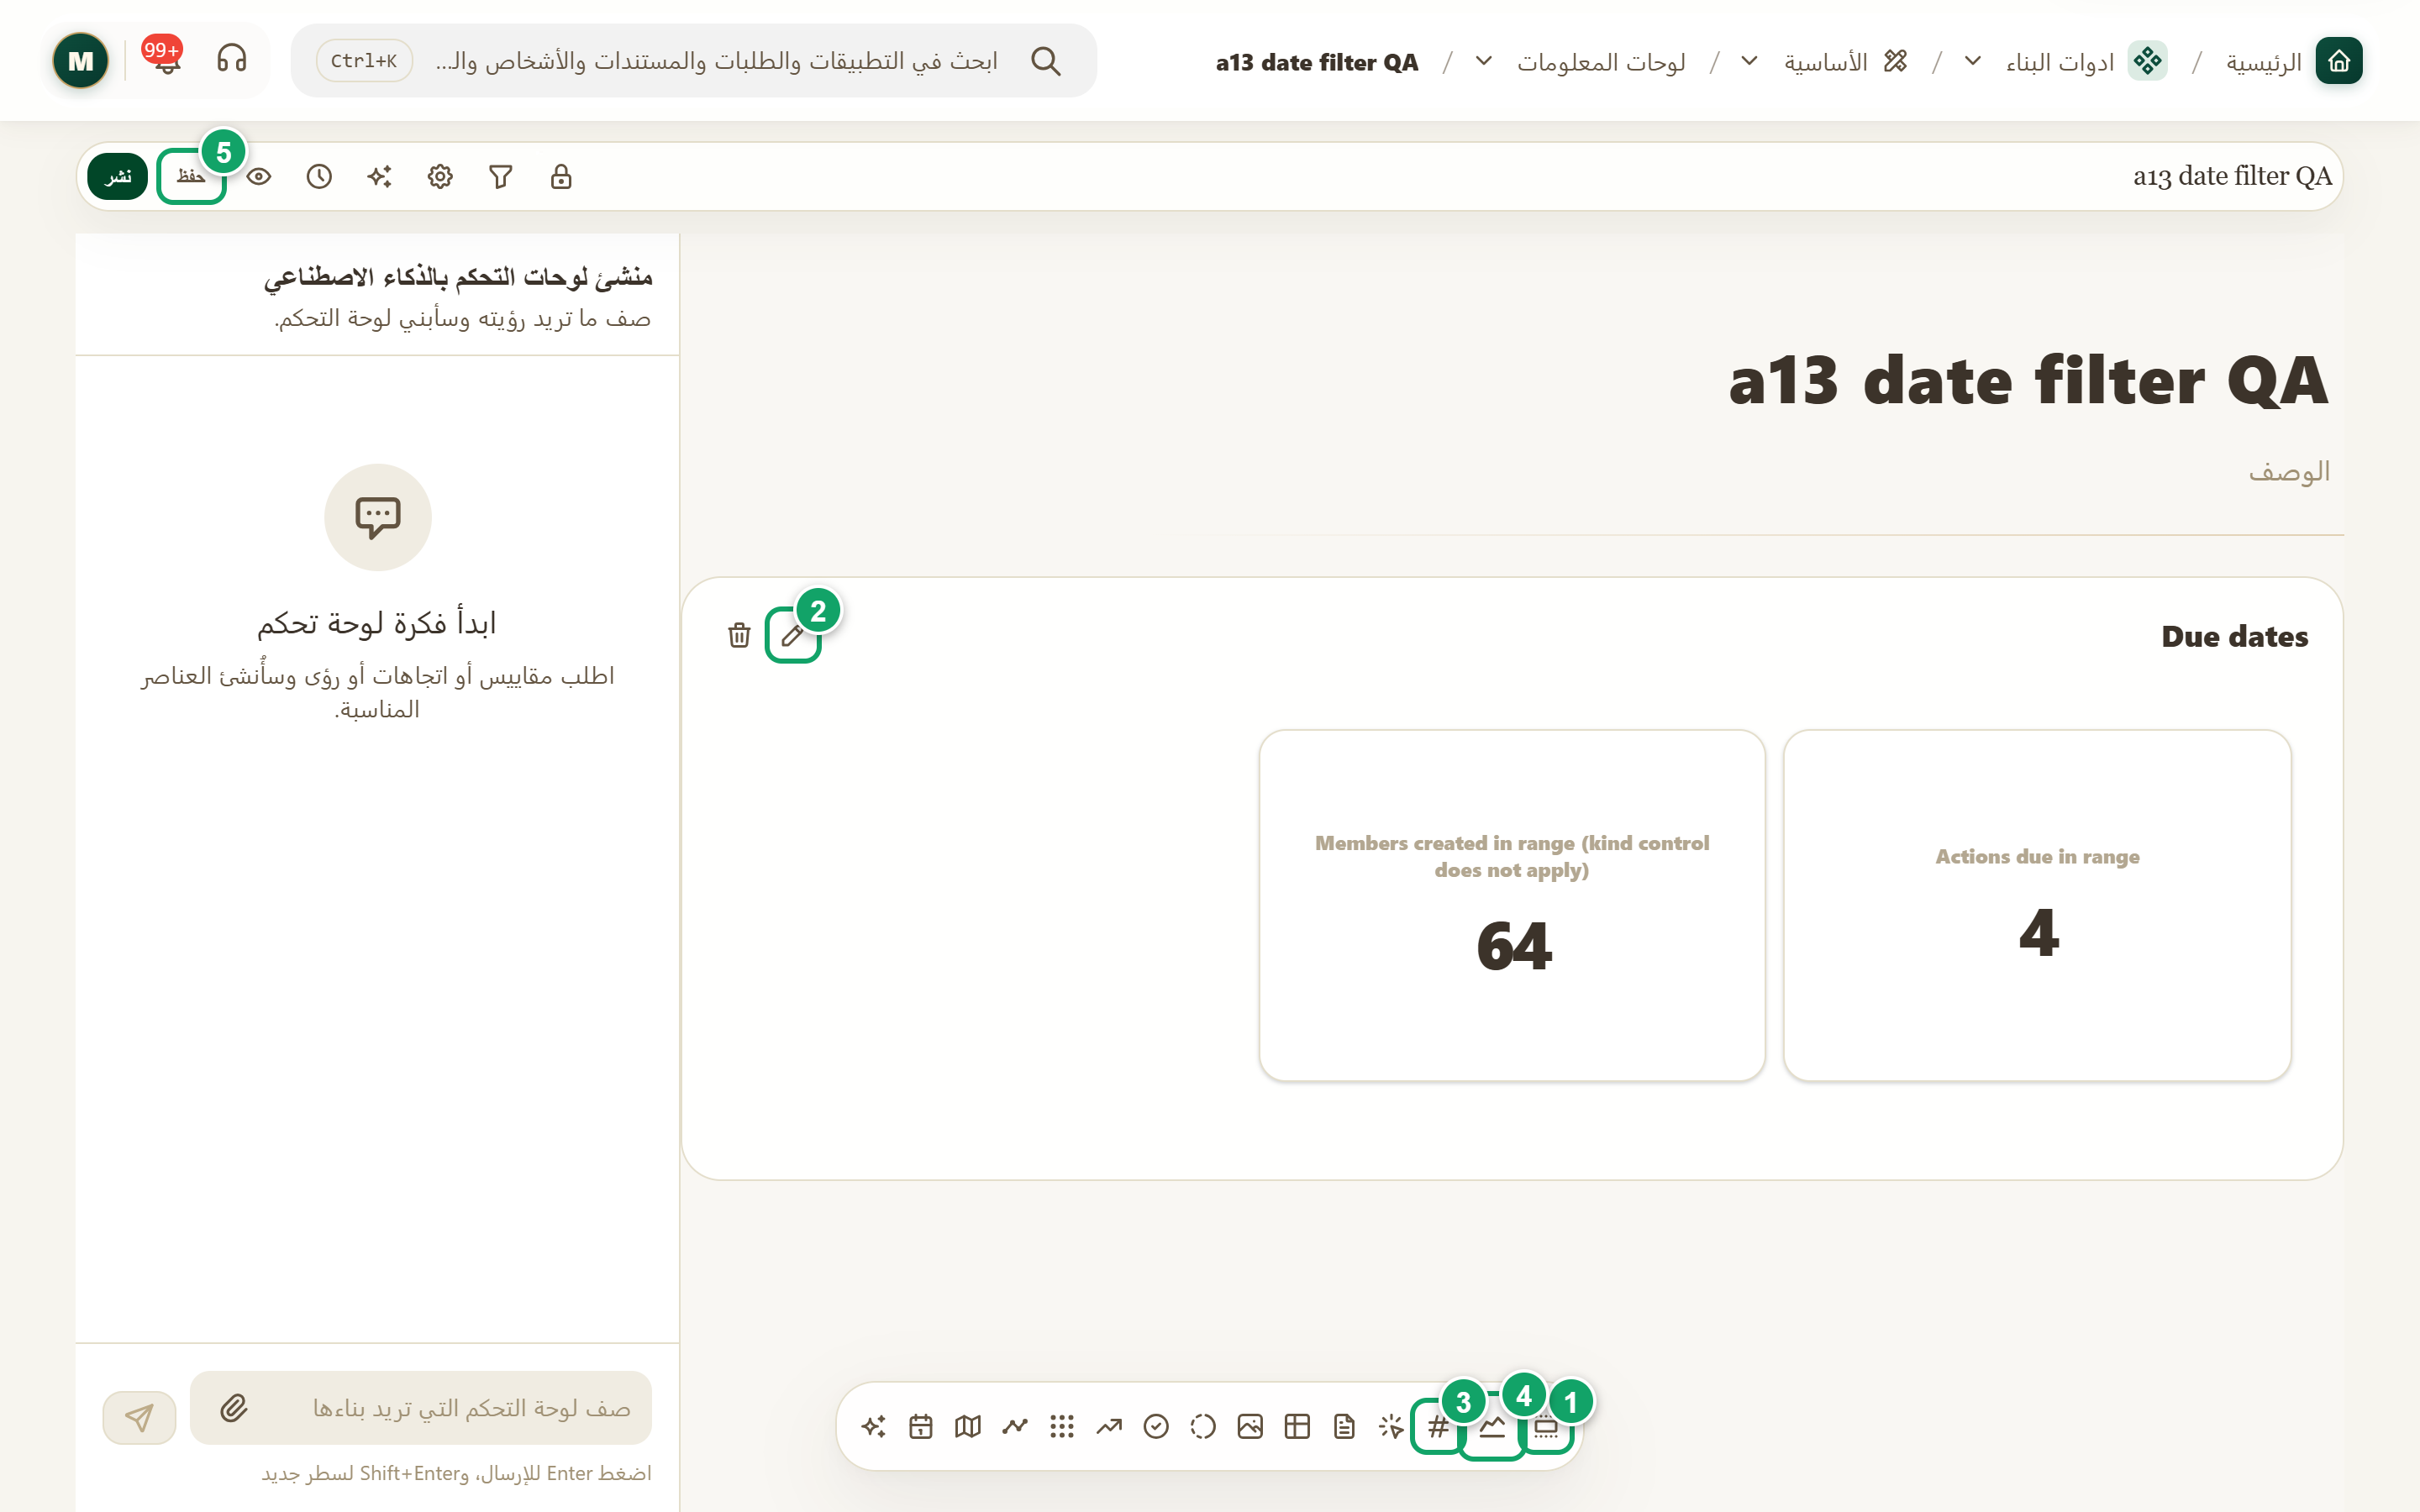
\includegraphics[width=0.95\linewidth,height=0.72\textheight,keepaspectratio]{figures/screens/ch06-dash-builder-ar.png}
\caption{منشئ اللوحة مع شريط الأدوات أسفل الصفحة}
\label{fig:builder-dashboards-builder-screen}
\shotnote{تعرض الصورة لوحة اختبار مفتوحة في المنشئ، فيها قسم واحد بعنصرين من نوع «رقم»، واللوحة الجانبية للذكاء الاصطناعي ظاهرة. ويجمع شريط الأدوات السفلي كل ما يضيف أقساماً وعناصر، بينما يجمع الرأس أزرار الضبط والحفظ. ① «إضافة قسم»: يضيف قسماً في آخر اللوحة. ② «تعديل»: زر القلم الذي يفتح عنوان القسم ووصفه. ③ «رقم»: يضيف عنصر رقم إلى آخر قسم. ④ زر الرسم البياني: يفتح قائمة «نوع الرسم البياني». ⑤ «حفظ»: يحفظ المسودة دون نشرها.}
\end{figure}

\begin{table}[H]
\centering
\caption{أزرار رأس المنشئ}
\label{tab:builder-dashboards-builder-header}
\begin{tabularx}{\linewidth}{R{3.6cm} Y}
\rcHeaderRow
\thh{الزر} & \thh{ما يفعله}\\
«إدارة الوصول» & يحدد من يستطيع فتح اللوحة، كما في صفحة «لوحات المعلومات».\\
«المرشحات» & يضيف المرشحات التي يغيّرها المشاهد، مثل نطاق التاريخ.\\
«الإعدادات» & يفتح إعدادات اللوحة: الاسم والوصف ومكان ظهورها في التنقل.\\
«منشئ لوحات التحكم بالذكاء الاصطناعي» & يُظهر اللوحة الجانبية التي تصف فيها ما تريد أو يخفيها، فيقترح الذكاء الاصطناعي العناصر.\\
«الإصدارات» و«معاينة» & يعرض الأول الإصدارات السابقة، ويعرض الثاني اللوحة كما يراها المشاهد.\\
«حفظ» و«نشر» & يحفظ الأول المسودة، ويحفظ الثاني ما في المنشئ ثم ينشره للمشاهدين.\\
\end{tabularx}
\end{table}

\begin{table}[H]
\centering
\caption{العمل على الأقسام والعناصر}
\label{tab:builder-dashboards-builder-grid}
\begin{tabularx}{\linewidth}{R{3.6cm} Y}
\rcHeaderRow
\thh{الإجراء} & \thh{كيف يتم}\\
إضافة قسم & اضغط «إضافة قسم» في شريط الأدوات أسفل الصفحة. ويُضاف القسم في آخر اللوحة.\\
تعديل القسم & اضغط زر القلم بجانب عنوانه، واكتب «عنوان القسم» و«الوصف»، ثم اضغط «حفظ». ويحذف زر سلة المهملات القسم.\\
إضافة عنصر & اضغط أيقونة نوع العنصر في شريط الأدوات، أو زر الرسم البياني لتختار من قائمة «نوع الرسم البياني». ويُضاف العنصر إلى آخر قسم، ويُضاف بجانب عنصر آخر إذا ضغطت علامة \en{+} عند حافته.\\
ترتيب العنصر & اسحبه داخل الشبكة أو غيّر حجمه من حافته. وتنقله قائمة «نقل العنصر» إلى الأعلى أو الأسفل أو الجانبين، أو إلى قسم آخر بأمر «نقل إلى القسم».\\
ضبط العنصر & اضغط العنصر لتفتح لوحة إعداداته، وفيها أيضاً «نسخ» لعمل نسخة منه و«حذف» لإزالته.\\
\end{tabularx}
\end{table}

\begin{rcwarn}[الرسم الجديد يبدأ ببيانات تجريبية]
يظهر الرسم البياني الجديد ببيانات تجريبية حتى تختار له مصدر بيانات حقيقياً. فلا تنشر اللوحة قبل أن تربط كل عنصر بمصدره، وإلا رأى المشاهدون أرقاماً لا تخص المؤسسة.
\end{rcwarn}

\begin{figure}[H]
\centering
\begin{tikzpicture}[node distance=0.5cm]
\node[stepBox] (a) {\RL{إضافة قسم}};
\node[stepBox,below=of a] (b) {\RL{إضافة عنصر إلى القسم}};
\node[stepBox,below=of b] (c) {\RL{ضبط العنصر من لوحة إعداداته}};
\node[stepBox,below=of c] (d) {\RL{ترتيب العناصر وتحديد أحجامها}};
\node[stepBox,below=of d] (e) {\RL{حفظ المسودة}};
\draw[flowsTo] (a) -- (b);
\draw[flowsTo] (b) -- (c);
\draw[flowsTo] (c) -- (d);
\draw[flowsTo] (d) -- (e);
\end{tikzpicture}
\rclegend
\caption{بناء محتوى اللوحة}
\label{fig:builder-dashboards-builder-flow}
\shotnote{يبدأ المخطط بالقسم لأن كل عنصر ينتمي إلى قسم، والعنصر الجديد يذهب إلى آخر قسم في اللوحة. ويأتي الترتيب بعد الضبط، لأن حجم العنصر المناسب لا يتضح إلا بعد أن يعرض بياناته الحقيقية. وينتهي المخطط بالحفظ، لأن ترتيب العناصر لا يُحفظ في المسودة إلا بضغط «حفظ» أو «نشر».}
\end{figure}

\subsection{خطوات العمل والتحقق}
\begin{enumerate}
\item افتح اللوحة في المنشئ، واضغط «إضافة قسم»، ثم اضغط زر القلم واكتب «عنوان القسم» واضغط «حفظ».
\item اضغط أيقونة «رقم» في شريط الأدوات، ثم زر الرسم البياني واختر «دائري» من «نوع الرسم البياني».
\item اضغط كل عنصر واضبط مصدر بياناته كما في صفحة «إعدادات العنصر ومصادر بياناته».
\item اسحب العناصر وغيّر أحجامها حتى يصبح القسم مقروءاً، ثم اضغط «حفظ».
\end{enumerate}

\textbf{تحقق ومعالجة المشكلة:} يجب أن تبقى الأقسام والعناصر في أماكنها بعد إعادة فتح المنشئ. فإذا اختفى عنصر أضفته، فابحث عنه في آخر قسم من اللوحة، ثم انقله بأمر «نقل إلى القسم». وإذا عرض رسم أرقاماً غريبة، فمصدره ما زال البيانات التجريبية.

\clearpage
\section{إعدادات العنصر ومصادر بياناته}
\label{sec:builder-feature-dashboards-widget-settings}

عندما تضغط عنصراً في المنشئ تُفتح لوحة إعداداته، وفيها ثلاثة تبويبات: «عام» للعنوان والحجم، و«البيانات» لمصدر الأرقام وطريقة حسابها، و«النمط» للألوان والشكل. ويحدد مصدر البيانات من أين يأخذ العنصر أرقامه، ويحدد «مستوى الوصول» هل يرى كل مشاهد ما تسمح به صلاحياته فقط.

\textbf{المسار ومن يستخدمه:} منشئ اللوحة ← اضغط العنصر ← لوحة الإعدادات. يستخدمها من يبني اللوحة، ويُفتح تبويب «البيانات» أولاً.

\begin{rcnote}[مثال: شركة الأفق]
يختار مسؤول النظام لعنصر الطلبات المنتظرة المصدر «كيان» ونوع السجلات «طلبات الزيارة»، ونوع القيمة «عدد»، ثم يضيف مرشحاً يقصر العدّ على الطلبات التي تنتظر المراجعة. ويختار «حسب صلاحيات المستخدم» فترى سارة الخطيب طلبات فروعها فقط.
\end{rcnote}

\begin{figure}[H]
\centering
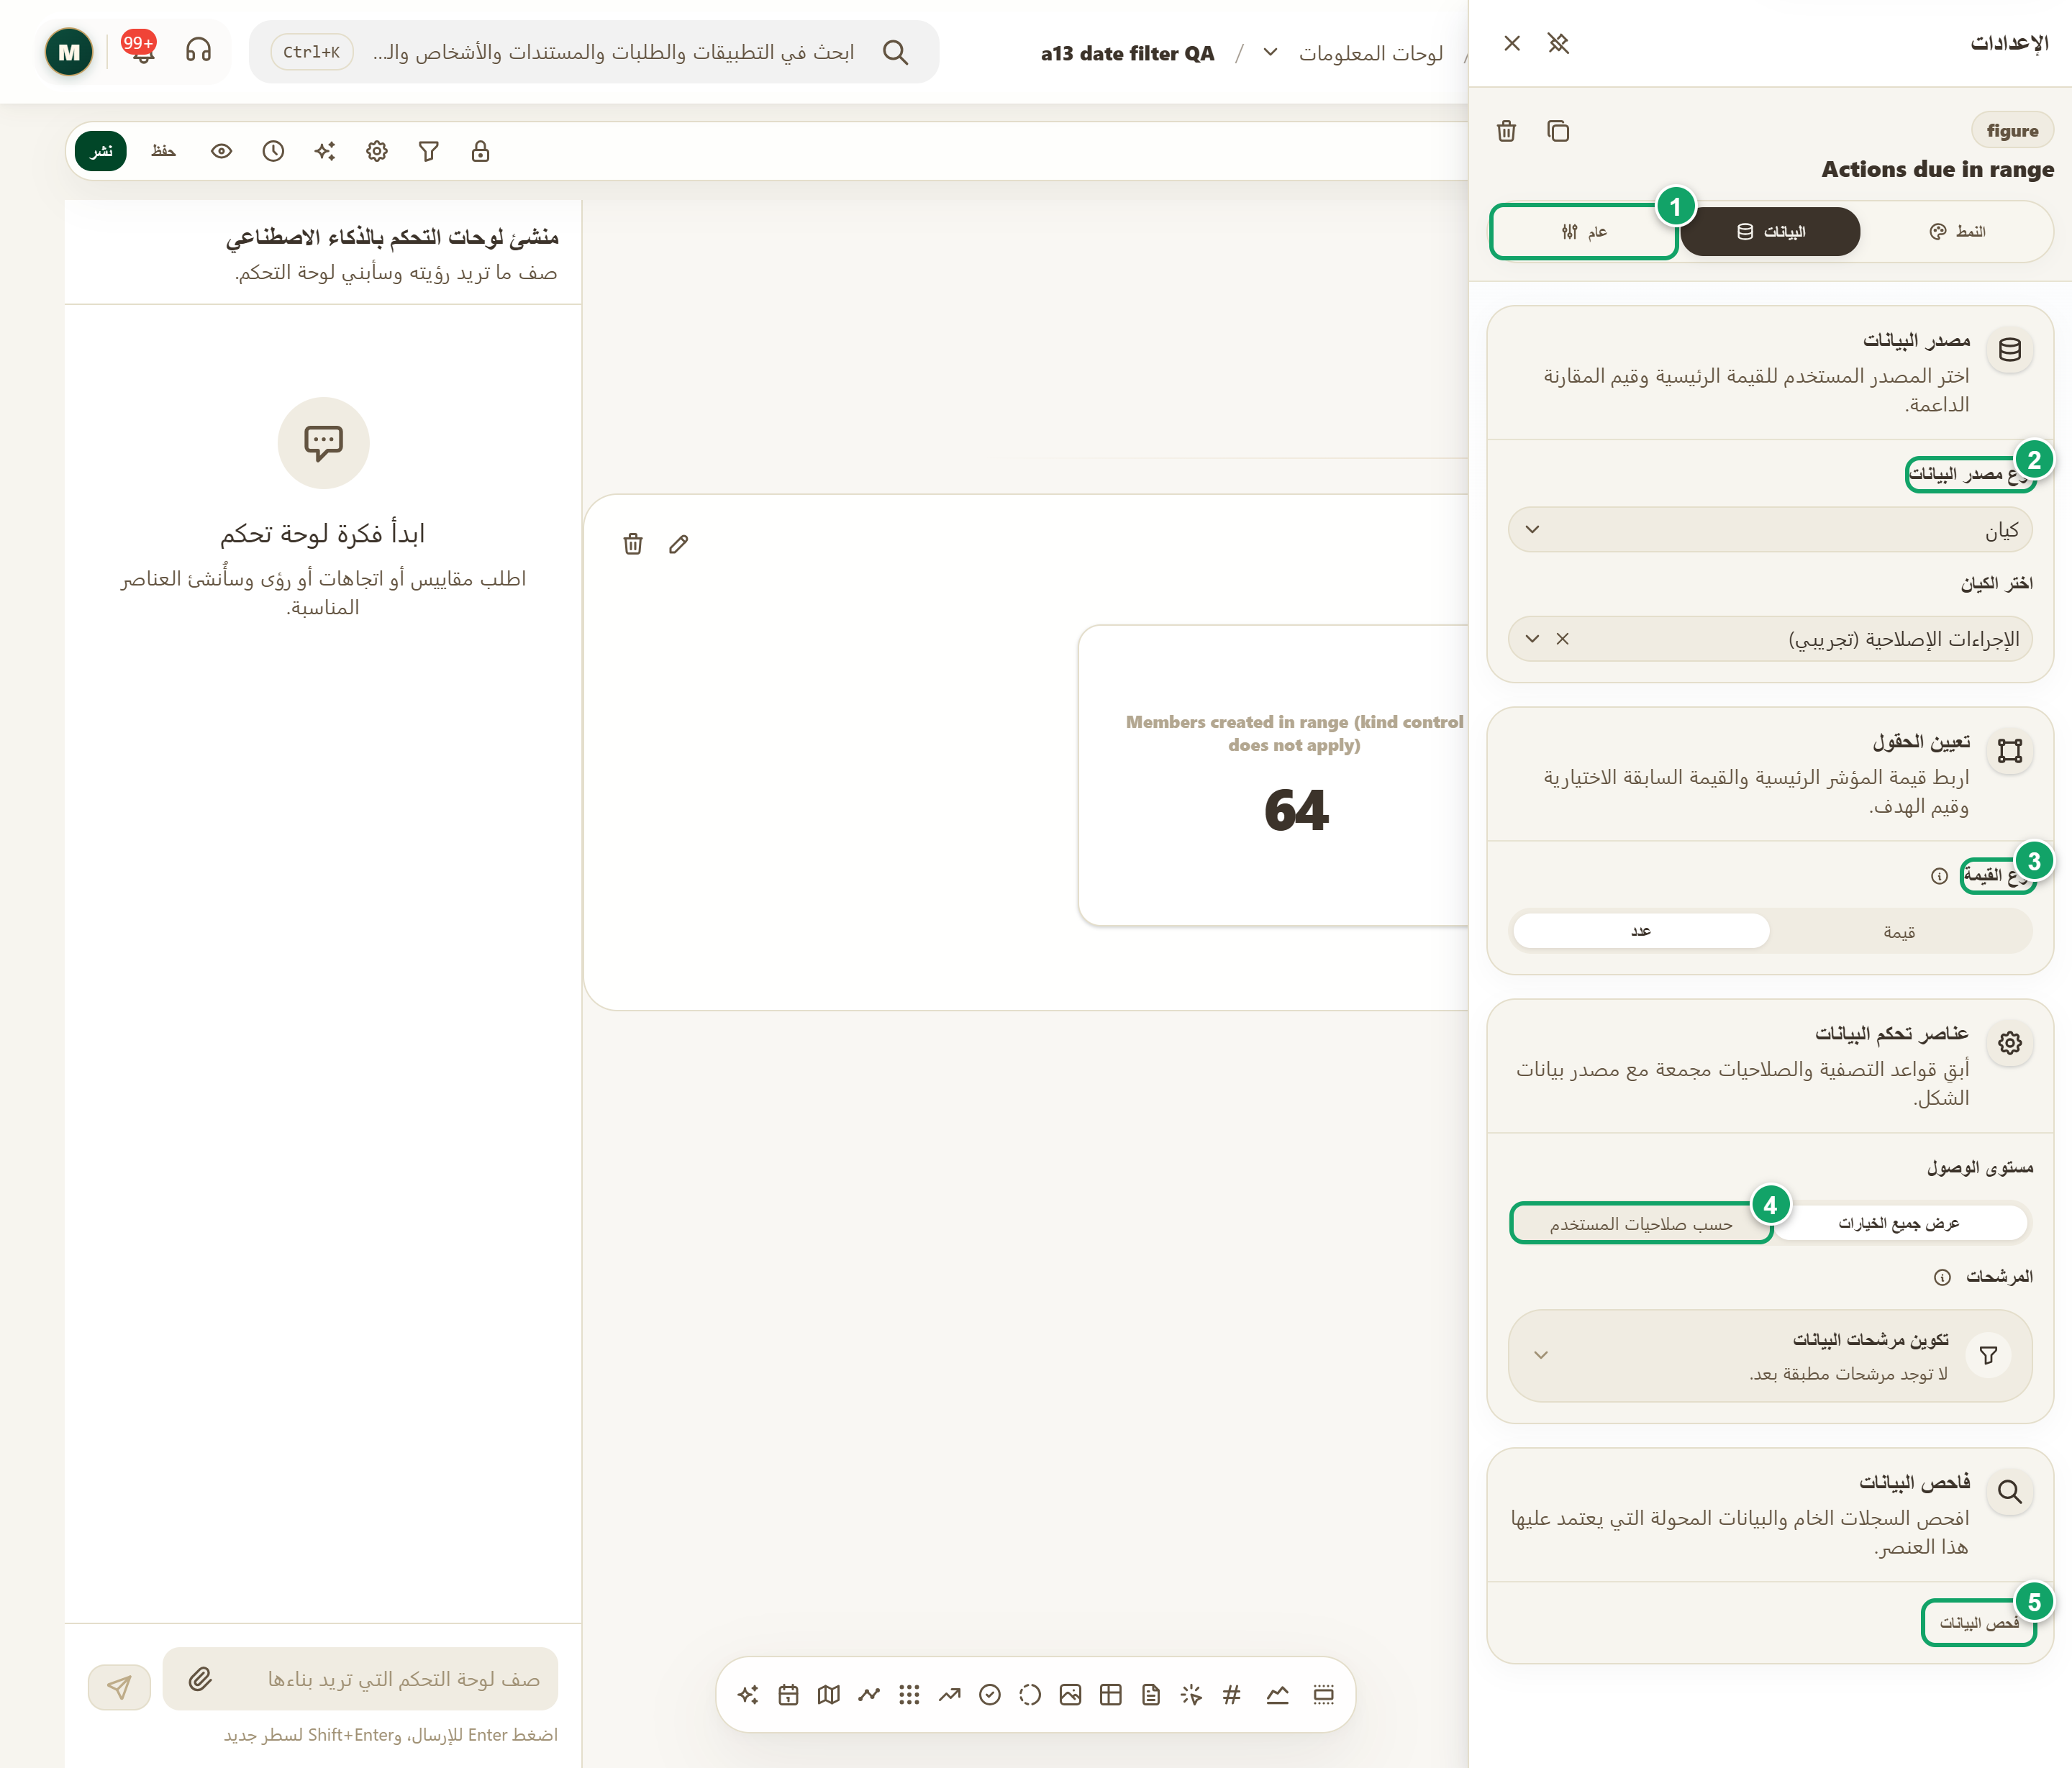
\includegraphics[width=0.95\linewidth,height=0.72\textheight,keepaspectratio]{figures/screens/ch06-dash-widget-settings-ar.png}
\caption{لوحة إعدادات عنصر «رقم» على تبويب «البيانات»}
\label{fig:builder-dashboards-widget-settings-screen}
\shotnote{تعرض الصورة لوحة الإعدادات بعد الضغط على عنصر «رقم» في لوحة اختبار، وقد فُتح تبويب «البيانات» تلقائياً. وفي هذا النوع يسمى قسم الصلاحيات والمرشحات «عناصر تحكم البيانات»، ويظهر فيه «مستوى الوصول» الذي يحدد ما يراه كل مشاهد. ① «عام»: العنوان والعرض والارتفاع. ② «نوع مصدر البيانات»: من أين يأخذ العنصر أرقامه. ③ «نوع القيمة»: «عدد» أو «قيمة». ④ «حسب صلاحيات المستخدم»: يحسب الرقم بصلاحيات من يفتح اللوحة. ⑤ «فحص البيانات»: يعرض السجلات التي قرأها العنصر.}
\end{figure}

\begin{table}[H]
\centering
\caption{مصادر البيانات في «نوع مصدر البيانات»}
\label{tab:builder-dashboards-widget-settings-sources}
\begin{tabularx}{\linewidth}{R{3.6cm} Y}
\rcHeaderRow
\thh{المصدر} & \thh{متى تستخدمه}\\
«كيان» & المصدر المعتاد: تختار نوع السجلات من «اختر الكيان»، ثم الحقول التي يعرضها العنصر أو يعدّها.\\
«إجراء تشغيلي» & يستدعي العنصر مشغّل ويب هوك في مسار إجراء تشغيلي ويعرض ما يعيده، ويجرّبه زر «اختبار SOP».\\
«خطة تكليف» & يعرض أرقام خطة تكليف وجولاتها، مثل عدد المهام المُسندة والمنجزة والمتأخرة.\\
«الفحوص والنتائج» & يعرض فحوص الجودة في نموذج تختاره: درجات الطلبات، أو الفحوص، أو نتائج الذكاء الاصطناعي.\\
«بيانات يدوية» & تكتب البيانات بنفسك بصيغة \en{JSON}، وتناسب مثالاً ثابتاً أو رقماً لا يُحفظ في النظام.\\
«المراسلات الرسمية» & يظهر لمن يملك تطبيق المراسلات، ويعرض الرسائل أو الأعمال أو السجل أو الأداء في فترة تختارها.\\
\end{tabularx}
\end{table}

\begin{table}[H]
\centering
\caption{ما تضبطه في التبويبات الثلاثة}
\label{tab:builder-dashboards-widget-settings-tabs}
\begin{tabularx}{\linewidth}{R{3.6cm} Y}
\rcHeaderRow
\thh{التبويب} & \thh{الإعدادات}\\
«عام» & «العنوان» الظاهر فوق العنصر، و«العرض» و«الارتفاع» بعدد خانات الشبكة.\\
«البيانات» & المصدر، ثم الحقول، و«نوع القيمة»: «عدد» لعدّ السجلات أو «قيمة» لحقل رقمي مع «التجميع» كالمجموع أو المتوسط.\\
«خيارات متقدمة ومرشحات» & داخل «البيانات»، وتسمى «عناصر تحكم البيانات» في عنصر «رقم»: «مستوى الوصول» بخياري «عرض جميع الخيارات» و«حسب صلاحيات المستخدم»، والمرشحات التي تضيّق السجلات، وخيار إخفاء العنصر عمّن لا يملك صلاحية.\\
«فاحص البيانات» & داخل «البيانات» أيضاً: يعرض زر «فحص البيانات» السجلات التي قرأها العنصر والبيانات بعد تحويلها، فتعرف سبب رقم غير متوقع.\\
«النمط» & الألوان والتسميات والخطوط وطريقة العرض. وتختلف خياراته بحسب نوع العنصر.\\
\end{tabularx}
\end{table}

\begin{rcwarn}[«عرض جميع الخيارات» يتجاوز صلاحيات المشاهد]
إذا اخترت «عرض جميع الخيارات» فسيرى كل من يفتح اللوحة أرقام جميع السجلات، حتى التي لا يستطيع فتحها. فاختر «حسب صلاحيات المستخدم» ما لم تكن الأرقام الكاملة مقصودة لكل من يصل إلى اللوحة.
\end{rcwarn}

\begin{figure}[H]
\centering
\begin{tikzpicture}[node distance=0.5cm]
\node[stepBox] (a) {\RL{اختيار نوع مصدر البيانات}};
\node[stepBox,below=of a] (b) {\RL{اختيار الكيان والحقول}};
\node[stepBox,below=of b] (c) {\RL{نوع القيمة والتجميع}};
\node[stepBox,below=of c] (d) {\RL{مستوى الوصول والمرشحات}};
\node[stepBox,below=of d] (e) {\RL{فاحص البيانات}};
\draw[flowsTo] (a) -- (b);
\draw[flowsTo] (b) -- (c);
\draw[flowsTo] (c) -- (d);
\draw[flowsTo] (d) -- (e);
\end{tikzpicture}
\rclegend
\caption{ضبط بيانات عنصر}
\label{fig:builder-dashboards-widget-settings-flow}
\shotnote{يتبع المخطط ترتيب تبويب «البيانات»: فالحقول المتاحة تعتمد على المصدر والكيان، والتجميع يعتمد على الحقل. ويأتي «فاحص البيانات» أخيراً لأنه يكشف أثر المرشحات ومستوى الوصول على الرقم قبل أن يراه أحد.}
\end{figure}

\subsection{خطوات العمل والتحقق}
\begin{enumerate}
\item اضغط العنصر في المنشئ، واكتب «العنوان» في تبويب «عام»، ثم اضبط «العرض» و«الارتفاع».
\item افتح «البيانات»، واختر «كيان» في «نوع مصدر البيانات»، ثم اختر نوع السجلات من «اختر الكيان».
\item اختر «عدد» أو «قيمة» في «نوع القيمة»، وحدد الحقل و«التجميع» عند الحاجة.
\item افتح «خيارات متقدمة ومرشحات»، واختر «حسب صلاحيات المستخدم»، وأضف المرشحات التي تقصر السجلات على ما تريد.
\item اضغط «فحص البيانات» وقارن السجلات المعروضة بما تعرفه، ثم اضبط الألوان في «النمط».
\end{enumerate}

\textbf{تحقق ومعالجة المشكلة:} يجب أن يطابق الرقم عدد السجلات التي تعرفها. فإذا ظهر «لا توجد بيانات»، فراجع المرشحات في «خيارات متقدمة ومرشحات». وإذا رأى مشاهد رسالة بأنه لا يملك صلاحية عرض البيانات، فهذا متوقع مع «حسب صلاحيات المستخدم»؛ فامنحه صلاحية قراءة النوع أو أخفِ العنصر عنه.

\clearpage
\section{أنواع العناصر}
\label{sec:builder-feature-dashboards-widgets}

يحدد نوع العنصر شكل عرض البيانات: رقم واحد، أو جدول، أو رسم بياني، أو تقويم، أو غير ذلك. ويضم شريط الأدوات في المنشئ ثلاثة عشر نوعاً، ويفتح زر الرسم البياني قائمة بواحد وثلاثين نوعاً من الرسوم. واختر النوع الذي يجيب عن سؤال المشاهد بأبسط شكل.

\textbf{المسار ومن يستخدمه:} منشئ اللوحة ← شريط الأدوات أسفل الصفحة. يستخدمه من يبني اللوحة، ويظهر اسم كل نوع عند تمرير المؤشر فوق أيقونته.

\begin{rcnote}[مثال: شركة الأفق]
يستخدم مسؤول النظام في لوحة «متابعة الزيارات» عنصر «رقم» للطلبات المنتظرة، ورسماً «دائري» للطلبات حسب الحالة، ورسم «أعمدة» للزيارات حسب الفرع، وعنصر «تقويم» لمواعيد الزيارات في فرع حلب وغيره.
\end{rcnote}

\begin{figure}[H]
\centering
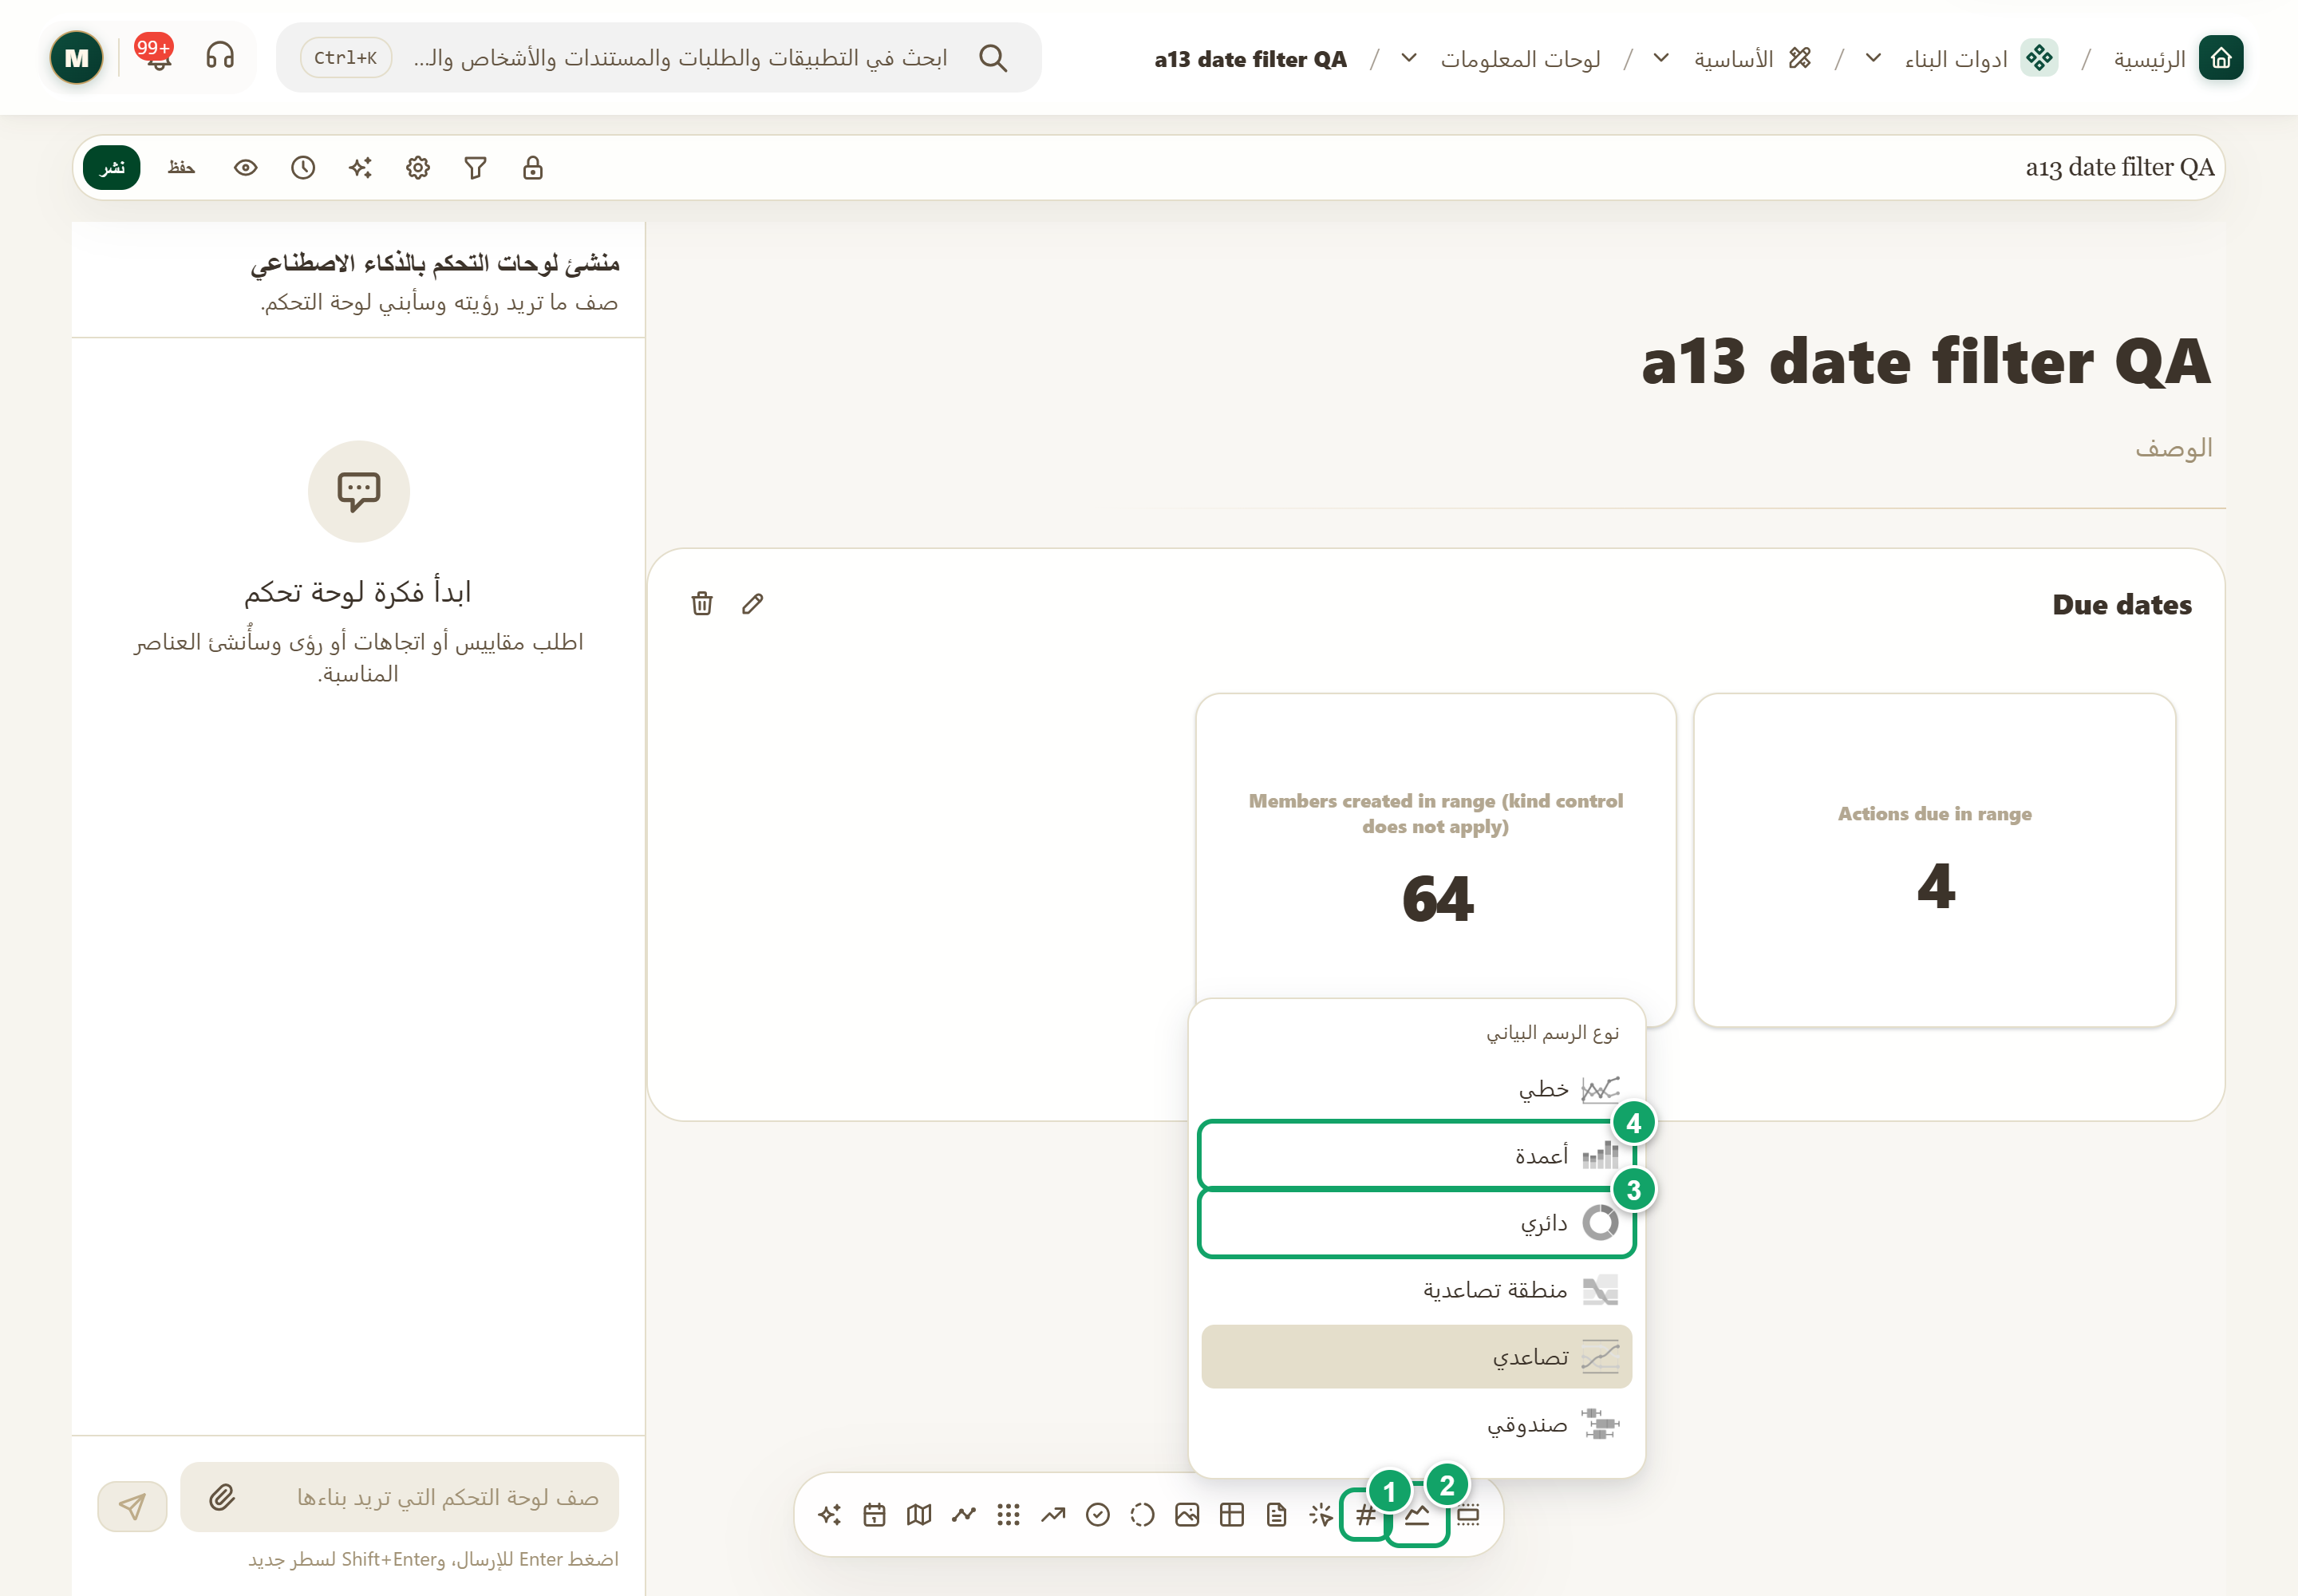
\includegraphics[width=0.95\linewidth,height=0.72\textheight,keepaspectratio]{figures/screens/ch06-dash-chart-types-ar.png}
\caption{قائمة «نوع الرسم البياني» فوق شريط الأدوات}
\label{fig:builder-dashboards-widgets-screen}
\shotnote{تعرض الصورة القائمة التي تفتح من زر الرسم البياني، وتظهر منها أوائل الرسوم، وتُعرض بقيتها بالتمرير داخل القائمة. أما الأنواع غير البيانية فلكل منها أيقونة مستقلة في شريط الأدوات يظهر اسمها عند تمرير المؤشر. ① «رقم»: أيقونة عنصر القيمة الواحدة. ② زر الرسم البياني: يفتح القائمة. ③ «دائري»: للأجزاء من الكل، مثل الطلبات حسب الحالة. ④ «أعمدة»: للمقارنة بين فئات، مثل الزيارات حسب الفرع.}
\end{figure}

\begin{table}[H]
\centering
\caption{أنواع العناصر في شريط الأدوات}
\label{tab:builder-dashboards-widgets-types}
\begin{tabularx}{\linewidth}{R{3.6cm} Y}
\rcHeaderRow
\thh{المجموعة} & \thh{الأنواع ومتى تستخدم كلاً منها}\\
الأساسية & «رقم» لقيمة واحدة مع قيمة سابقة أو هدف عند الحاجة، و«جدول» لعرض السجلات في أعمدة تختارها، و«نص» لنص ثابت أو قيمة من حقل، و«صورة» من رابط أو حقل، و«زر» ينقل إلى صفحة أو نموذج أو رابط.\\
الحالة والتقدم & «تقدم» لنسبة قيمة إلى حد أعلى، و«حالة» لشارة يتغير لونها بحسب قيمة حقل، و«مؤشر أداء» لقيمة رئيسية مع مقارنة وهدف وألوان حدود.\\
عناصر خاصة & «خريطة حرارية» لجدول صفوف وأعمدة تُلوَّن خلاياه بحسب القيمة، و«الجدول الزمني» لأحداث مرتبة بالتاريخ، و«خريطة» لمواقع السجلات، و«تقويم» لمواعيدها.\\
تحليل بالذكاء الاصطناعي & «تحليل الذكاء الاصطناعي» يقرأ صفوفاً من مصدر أو أكثر ويكتب تحليلاً بحسب «توجيه التحليل»، ثم يجيب عن أسئلة المتابعة.\\
\end{tabularx}
\end{table}

\begin{table}[H]
\centering
\caption{الرسوم البيانية في «نوع الرسم البياني»}
\label{tab:builder-dashboards-widgets-charts}
\begin{tabularx}{\linewidth}{R{3.6cm} Y}
\rcHeaderRow
\thh{الغرض} & \thh{الرسوم المناسبة}\\
المقارنة بين فئات & «أعمدة»، و«أعمدة قطبية»، و«أعمدة شعاعية»، و«رادار».\\
التغير مع الزمن & «خطي»، و«تدفق»، و«تصاعدي»، و«تقويم» يلوّن أيام السنة، و«نطاق زمني».\\
الأجزاء من الكل & «دائري»، و«وافل»، و«خريطة شجرية»، و«شعاعي متشعب»، و«دوائر متداخلة».\\
المراحل والتدفق & «قمع» لمراحل يتناقص عددها، و«سانكي» لانتقال الكميات بين المراحل.\\
التوزيع والعلاقة & «مبعثر»، و«صندوقي»، و«سرب نقاط»، و«خريطة حرارية»، و«إحداثيات متوازية».\\
الخرائط & «مناطق لونية» لتلوين المناطق بحسب القيمة، و«خريطة جغرافية» لرسم المناطق.\\
\end{tabularx}
\end{table}

وتبقى في القائمة رسوم متخصصة أخرى، مثل «وتري» و«شبكة» و«شجرة» و«جليدي». وتضبط مظهر أي رسم من «خيارات الرسم البياني» في تبويب «النمط»، وتعيدها إلى أصلها بزر «إعادة التعيين إلى الافتراضي».

\begin{figure}[H]
\centering
\begin{tikzpicture}[node distance=0.5cm]
\node[stepBox] (a) {\RL{ما السؤال الذي يجيب عنه العنصر؟}};
\node[stepBox,below=of a] (b) {\RL{رقم واحد أم قائمة أم رسم؟}};
\node[stepBox,below=of b] (c) {\RL{اختيار النوع وإضافته}};
\node[stepBox,below=of c] (d) {\RL{ربطه بمصدر البيانات}};
\draw[flowsTo] (a) -- (b);
\draw[flowsTo] (b) -- (c);
\draw[flowsTo] (c) -- (d);
\end{tikzpicture}
\rclegend
\caption{اختيار نوع العنصر}
\label{fig:builder-dashboards-widgets-flow}
\shotnote{يبدأ المخطط بسؤال المشاهد لا بشكل الرسم، لأن النوع المناسب يتبع ما يريد المشاهد معرفته. فالعدد الحالي يكفيه «رقم»، والمقارنة بين الفروع تحتاج إلى «أعمدة»، والمواعيد تُفهم أسرع في «تقويم».}
\end{figure}

\subsection{خطوات العمل والتحقق}
\begin{enumerate}
\item اكتب السؤال الذي يجيب عنه العنصر، مثل «كم طلباً ينتظر المراجعة؟».
\item اختر من الجدولين النوع الذي يجيب عنه، ومرّر المؤشر فوق أيقونات شريط الأدوات حتى تجد اسمه.
\item اضغط الأيقونة، أو زر الرسم البياني ثم اسم الرسم في «نوع الرسم البياني».
\item اضبط مصدر البيانات والحقول المطلوبة لهذا النوع، ثم راجع شكله في «معاينة».
\end{enumerate}

\textbf{تحقق ومعالجة المشكلة:} يجب أن يجيب العنصر عن سؤاله من نظرة واحدة. فإذا ازدحم الرسم بفئات كثيرة، فاستخدم «جدول» أو أضف مرشحاً يقلل الفئات. وإذا لم يعرض «تحليل الذكاء الاصطناعي» نتيجة، فاضغط «إنشاء النتيجة»، لأن المنشئ يوقف التحليل أثناء التعديل.

\clearpage
\section{إعدادات اللوحة}
\label{sec:builder-feature-dashboards-settings}

تحدد إعدادات اللوحة اسمها ووصفها ومكان ظهورها في تنقل التطبيقات. وقد تظهر فيها أيضاً إعدادات تتحكم في البيانات التي يراها المشاهد، عندما تكون ميزات التنقل حسب العمل مفعّلة في المؤسسة.

\textbf{المسار ومن يستخدمه:} منشئ اللوحة ← «الإعدادات» ← نافذة «إعدادات لوحة المعلومات». يستخدمها من يبني اللوحة، ثم يضغط «حفظ».

\begin{rcnote}[مثال: شركة الأفق]
يفعّل مسؤول النظام «إظهار في التنقل» للوحة «متابعة الزيارات»، ويختار «خدمات الفروع» في «التطبيق» وقسم الزيارات في «قسم التطبيق»، فتظهر اللوحة لسارة الخطيب داخل التطبيق الذي تعمل فيه.
\end{rcnote}

\begin{figure}[H]
\centering
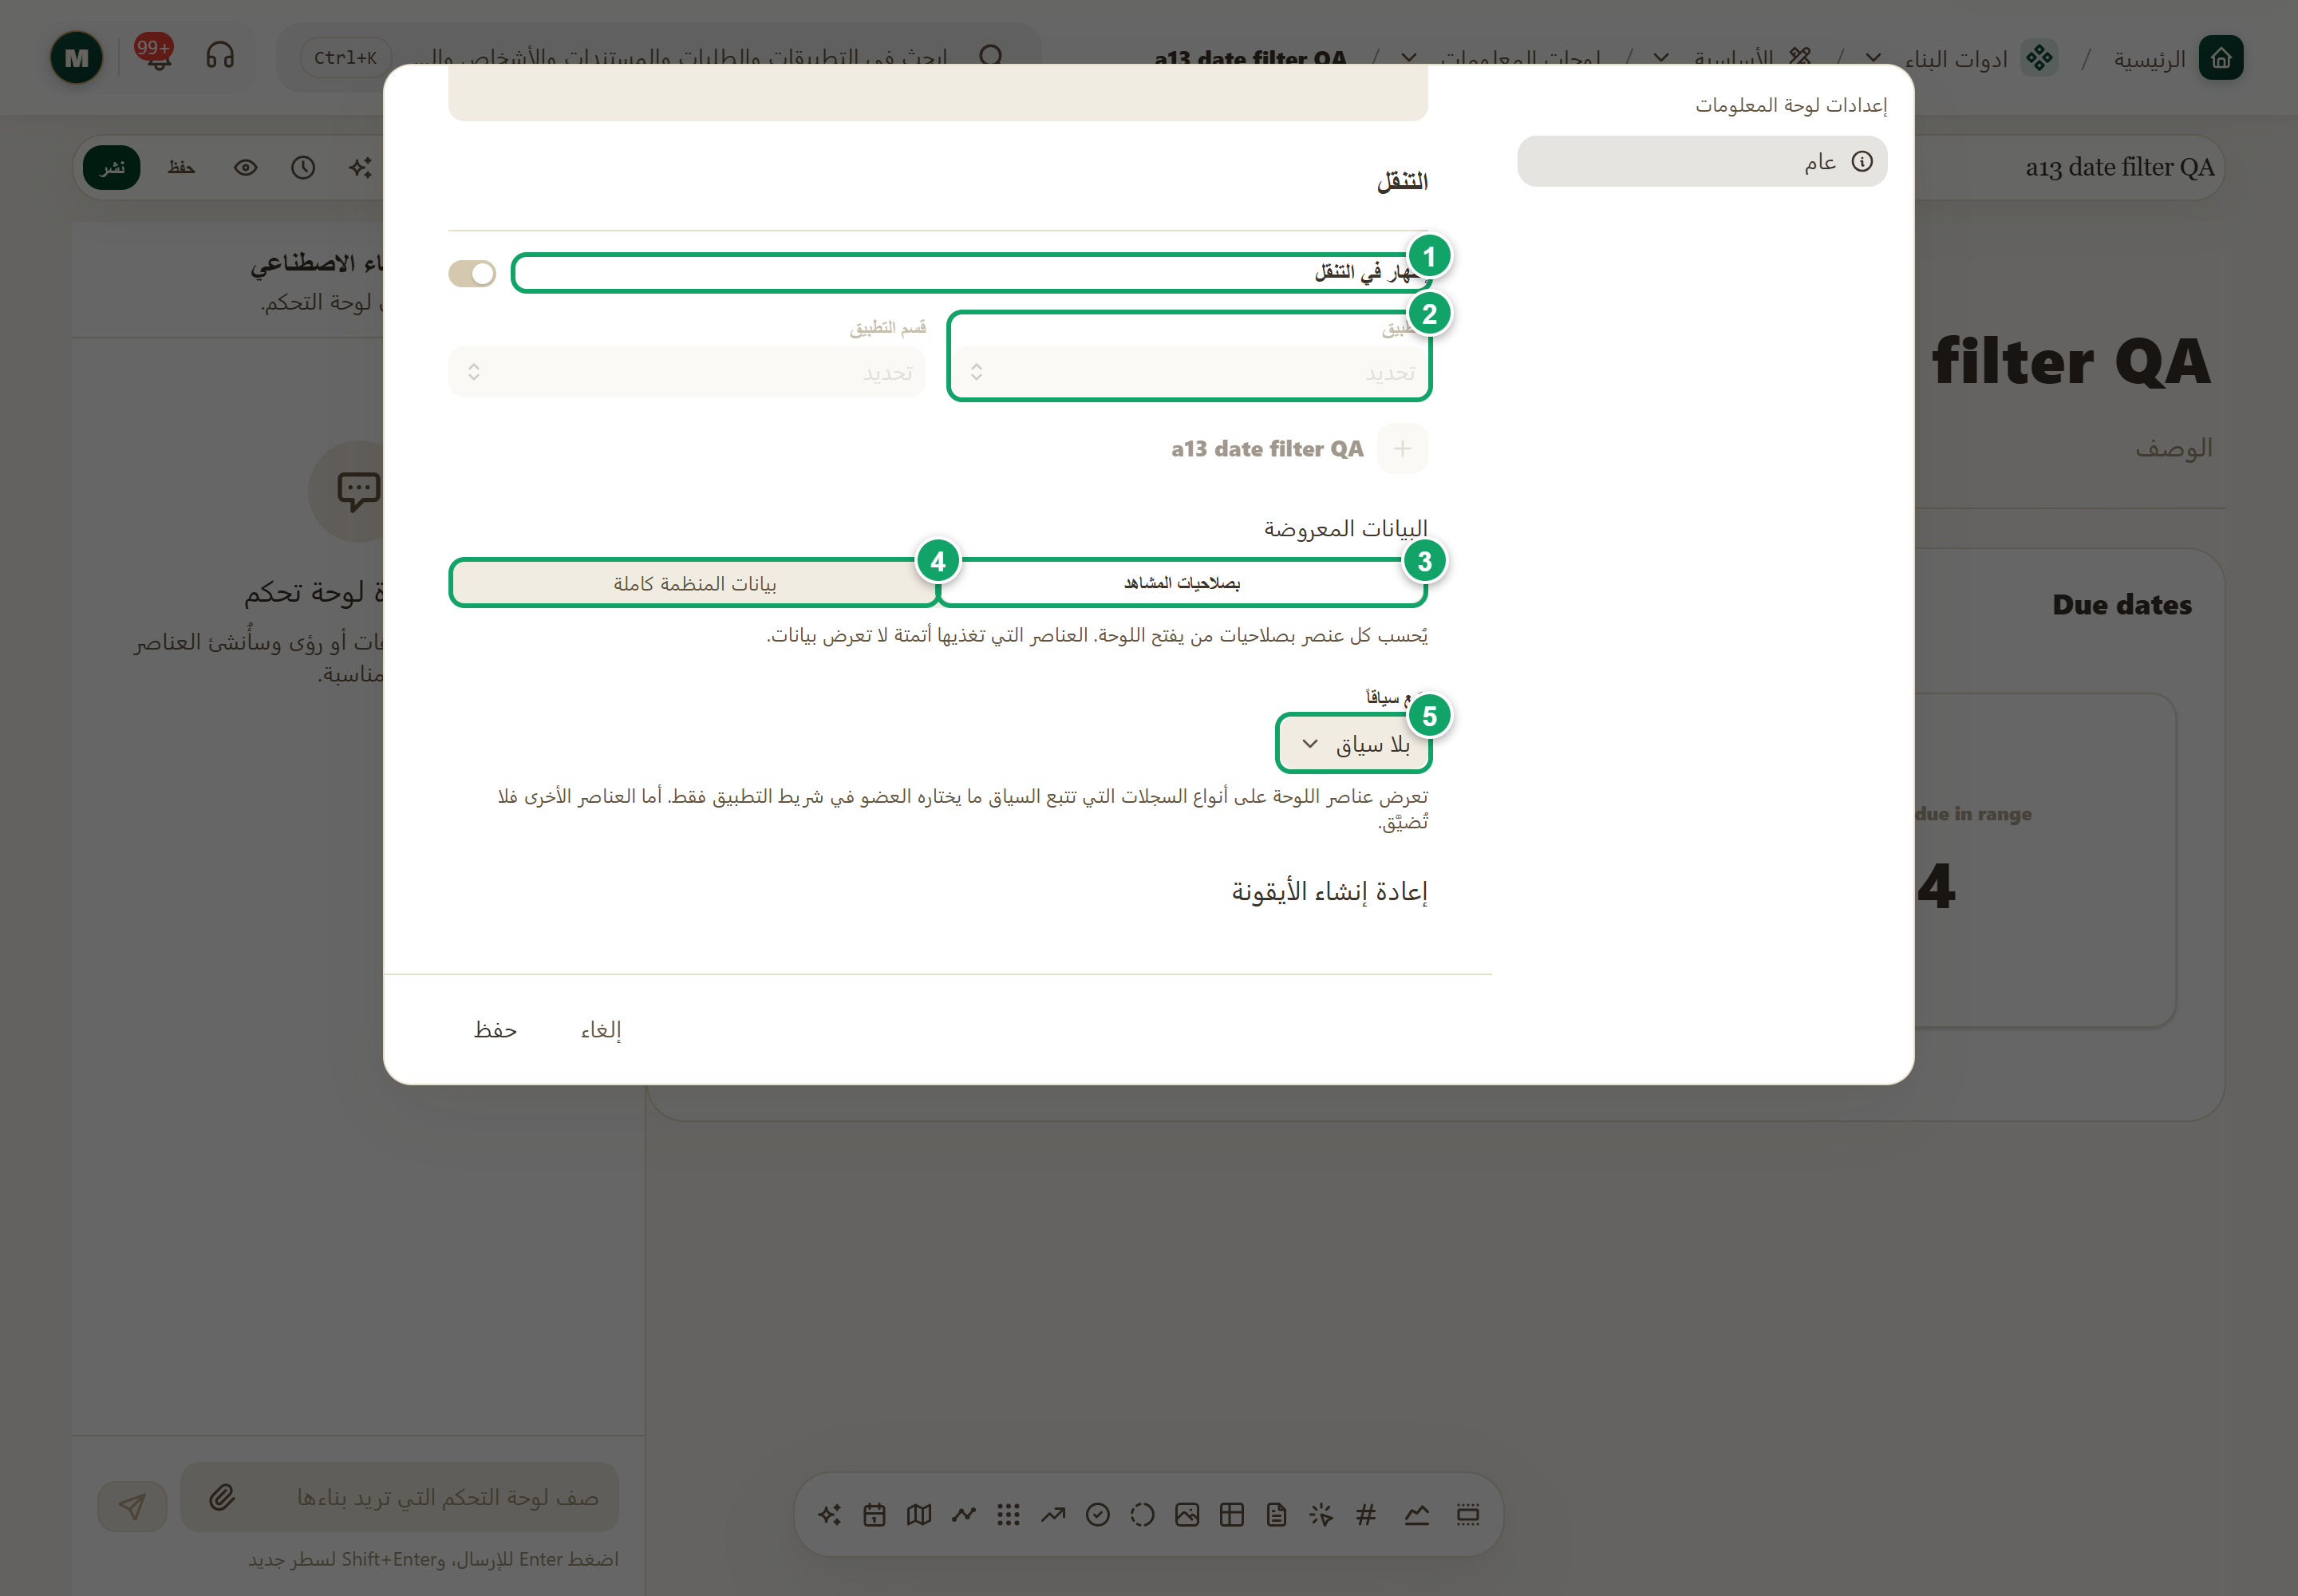
\includegraphics[width=0.95\linewidth,height=0.72\textheight,keepaspectratio]{figures/screens/ch06-dash-settings-ar.png}
\caption{نافذة «إعدادات لوحة المعلومات» بعد التمرير إلى قسم «التنقل»}
\label{fig:builder-dashboards-settings-screen}
\shotnote{تعرض الصورة نافذة إعدادات لوحة اختبار بعد التمرير إلى إعدادات الظهور والبيانات، والاسم والوصف أعلاها. ويظهر فيها «البيانات المعروضة» و«يتبع سياقاً» لأن هذه الميزات مفعّلة في مؤسسة الاختبار، وقد لا تظهر في مؤسستك. ① «إظهار في التنقل»: يضيف اللوحة إلى قائمة التطبيق. ② «التطبيق»: يتاح بعد التفعيل، ويليه «قسم التطبيق». ③ «بصلاحيات المشاهد»: الخيار الآمن الذي يحسب كل عنصر بصلاحيات من يفتح اللوحة. ④ «بيانات المنظمة كاملة»: يختاره مالك المؤسسة أو مسؤولها فقط. ⑤ «يتبع سياقاً»: يقصر العناصر على السياق المختار، و«بلا سياق» يتركها دون تضييق.}
\end{figure}

\begin{table}[H]
\centering
\caption{حقول «إعدادات لوحة المعلومات»}
\label{tab:builder-dashboards-settings-fields}
\begin{tabularx}{\linewidth}{R{3.6cm} Y}
\rcHeaderRow
\thh{الحقل} & \thh{المعنى}\\
«اسم لوحة المعلومات» و«الوصف» & الاسم الظاهر في القائمة والتنقل بكل لغة، ووصف قصير لما تتابعه اللوحة.\\
«إظهار في التنقل» & يضيف اللوحة عنصراً في قائمة التطبيق، مع أيقونة تختارها.\\
«التطبيق» و«قسم التطبيق» & التطبيق والقسم اللذان تظهر فيهما اللوحة.\\
«البيانات المعروضة» & «بصلاحيات المشاهد» فيُحسب كل عنصر بصلاحيات من يفتح اللوحة، أو «بيانات المنظمة كاملة» فيحتفظ كل عنصر بإعداد الوصول الخاص به. ولا يختار الخيار الثاني إلا مالك المؤسسة أو مسؤولها.\\
«يتبع سياقاً» & يقصر عناصر أنواع السجلات المرتبطة بسياق على ما يختاره العضو في شريط التطبيق، مثل فرع معين. والخيار «بلا سياق» يترك العناصر دون تضييق.\\
\end{tabularx}
\end{table}

\begin{rcwarn}[انتبه إلى «بيانات المنظمة كاملة»]
مع هذا الخيار يرى كل من يستطيع فتح اللوحة جميع السجلات في العناصر المضبوطة على «عرض جميع الخيارات»، ولو كانت صلاحياته أضيق. ولا تعرض العناصر التي تغذيها أتمتة أي بيانات مع «بصلاحيات المشاهد».
\end{rcwarn}

\begin{figure}[H]
\centering
\begin{tikzpicture}[node distance=0.5cm]
\node[stepBox] (a) {\RL{الاسم والوصف}};
\node[stepBox,below=of a] (b) {\RL{إظهار في التنقل}};
\node[stepBox,below=of b] (c) {\RL{التطبيق وقسم التطبيق}};
\node[stepBox,below=of c] (d) {\RL{البيانات المعروضة والسياق}};
\node[stepBox,below=of d] (e) {\RL{حفظ ثم نشر}};
\draw[flowsTo] (a) -- (b);
\draw[flowsTo] (b) -- (c);
\draw[flowsTo] (c) -- (d);
\draw[flowsTo] (d) -- (e);
\end{tikzpicture}
\rclegend
\caption{ضبط إعدادات اللوحة}
\label{fig:builder-dashboards-settings-flow}
\shotnote{يجمع المخطط قرارين: أين تظهر اللوحة، وأي بيانات يراها من يفتحها. ويُحسم مكان الظهور أولاً لأن السياق المقترح يعتمد على التطبيق والقسم، ثم يُحفظ كل ذلك وتُنشر اللوحة ليصل التغيير إلى المشاهدين.}
\end{figure}

\subsection{خطوات العمل والتحقق}
\begin{enumerate}
\item في المنشئ اضغط «الإعدادات»، وراجع «اسم لوحة المعلومات» و«الوصف».
\item فعّل «إظهار في التنقل»، واختر «التطبيق» ثم «قسم التطبيق» وأيقونة مناسبة.
\item إذا ظهر «البيانات المعروضة»، فاختر «بصلاحيات المشاهد» ما لم تحتج إلى غير ذلك.
\item إذا ظهر «يتبع سياقاً»، فاختر السياق الذي تتبعه اللوحة أو «بلا سياق»، ثم اضغط «حفظ» وانشر اللوحة.
\end{enumerate}

\textbf{تحقق ومعالجة المشكلة:} يجب أن تظهر اللوحة في القسم المختار من التطبيق. فإذا لم تظهر، فتأكد أن «إظهار في التنقل» مفعّل وأن اللوحة منشورة. وإذا رُفض اختيار «بيانات المنظمة كاملة»، فلا يختاره إلا مالك المؤسسة أو مسؤولها.

\clearpage
\section{مرشحات المشاهد ومحددات الكيانات}
\label{sec:builder-feature-dashboards-filters}

مرشحات المشاهد أدوات تظهر أعلى اللوحة، يغيّر بها المشاهد ما تعرضه العناصر دون أن يعدّل اللوحة. وتتيح ثلاثة أنواع: «نطاق التاريخ» لتحديد فترة، و«محدد» لاختيار سجل من نوع سجلات مثل فرع، و«اختر الحقل» لاختيار قيمة من قائمة خيارات. ولكل مرشح «النطاق» الذي يحدد العناصر التي يؤثر فيها.

\textbf{المسار ومن يستخدمه:} منشئ اللوحة ← «المرشحات». يضبطها من يبني اللوحة، ويستخدمها كل من يفتح اللوحة.

\begin{rcnote}[مثال: شركة الأفق]
يضيف مسؤول النظام إلى لوحة «متابعة الزيارات» مرشح «نطاق التاريخ» على تاريخ الزيارة، ومرشح «محدد» للفروع. فتختار سارة الخطيب فرع حلب والشهر الماضي، فتعرض كل العناصر زيارات ذلك الفرع في تلك الفترة.
\end{rcnote}

\begin{figure}[H]
\centering
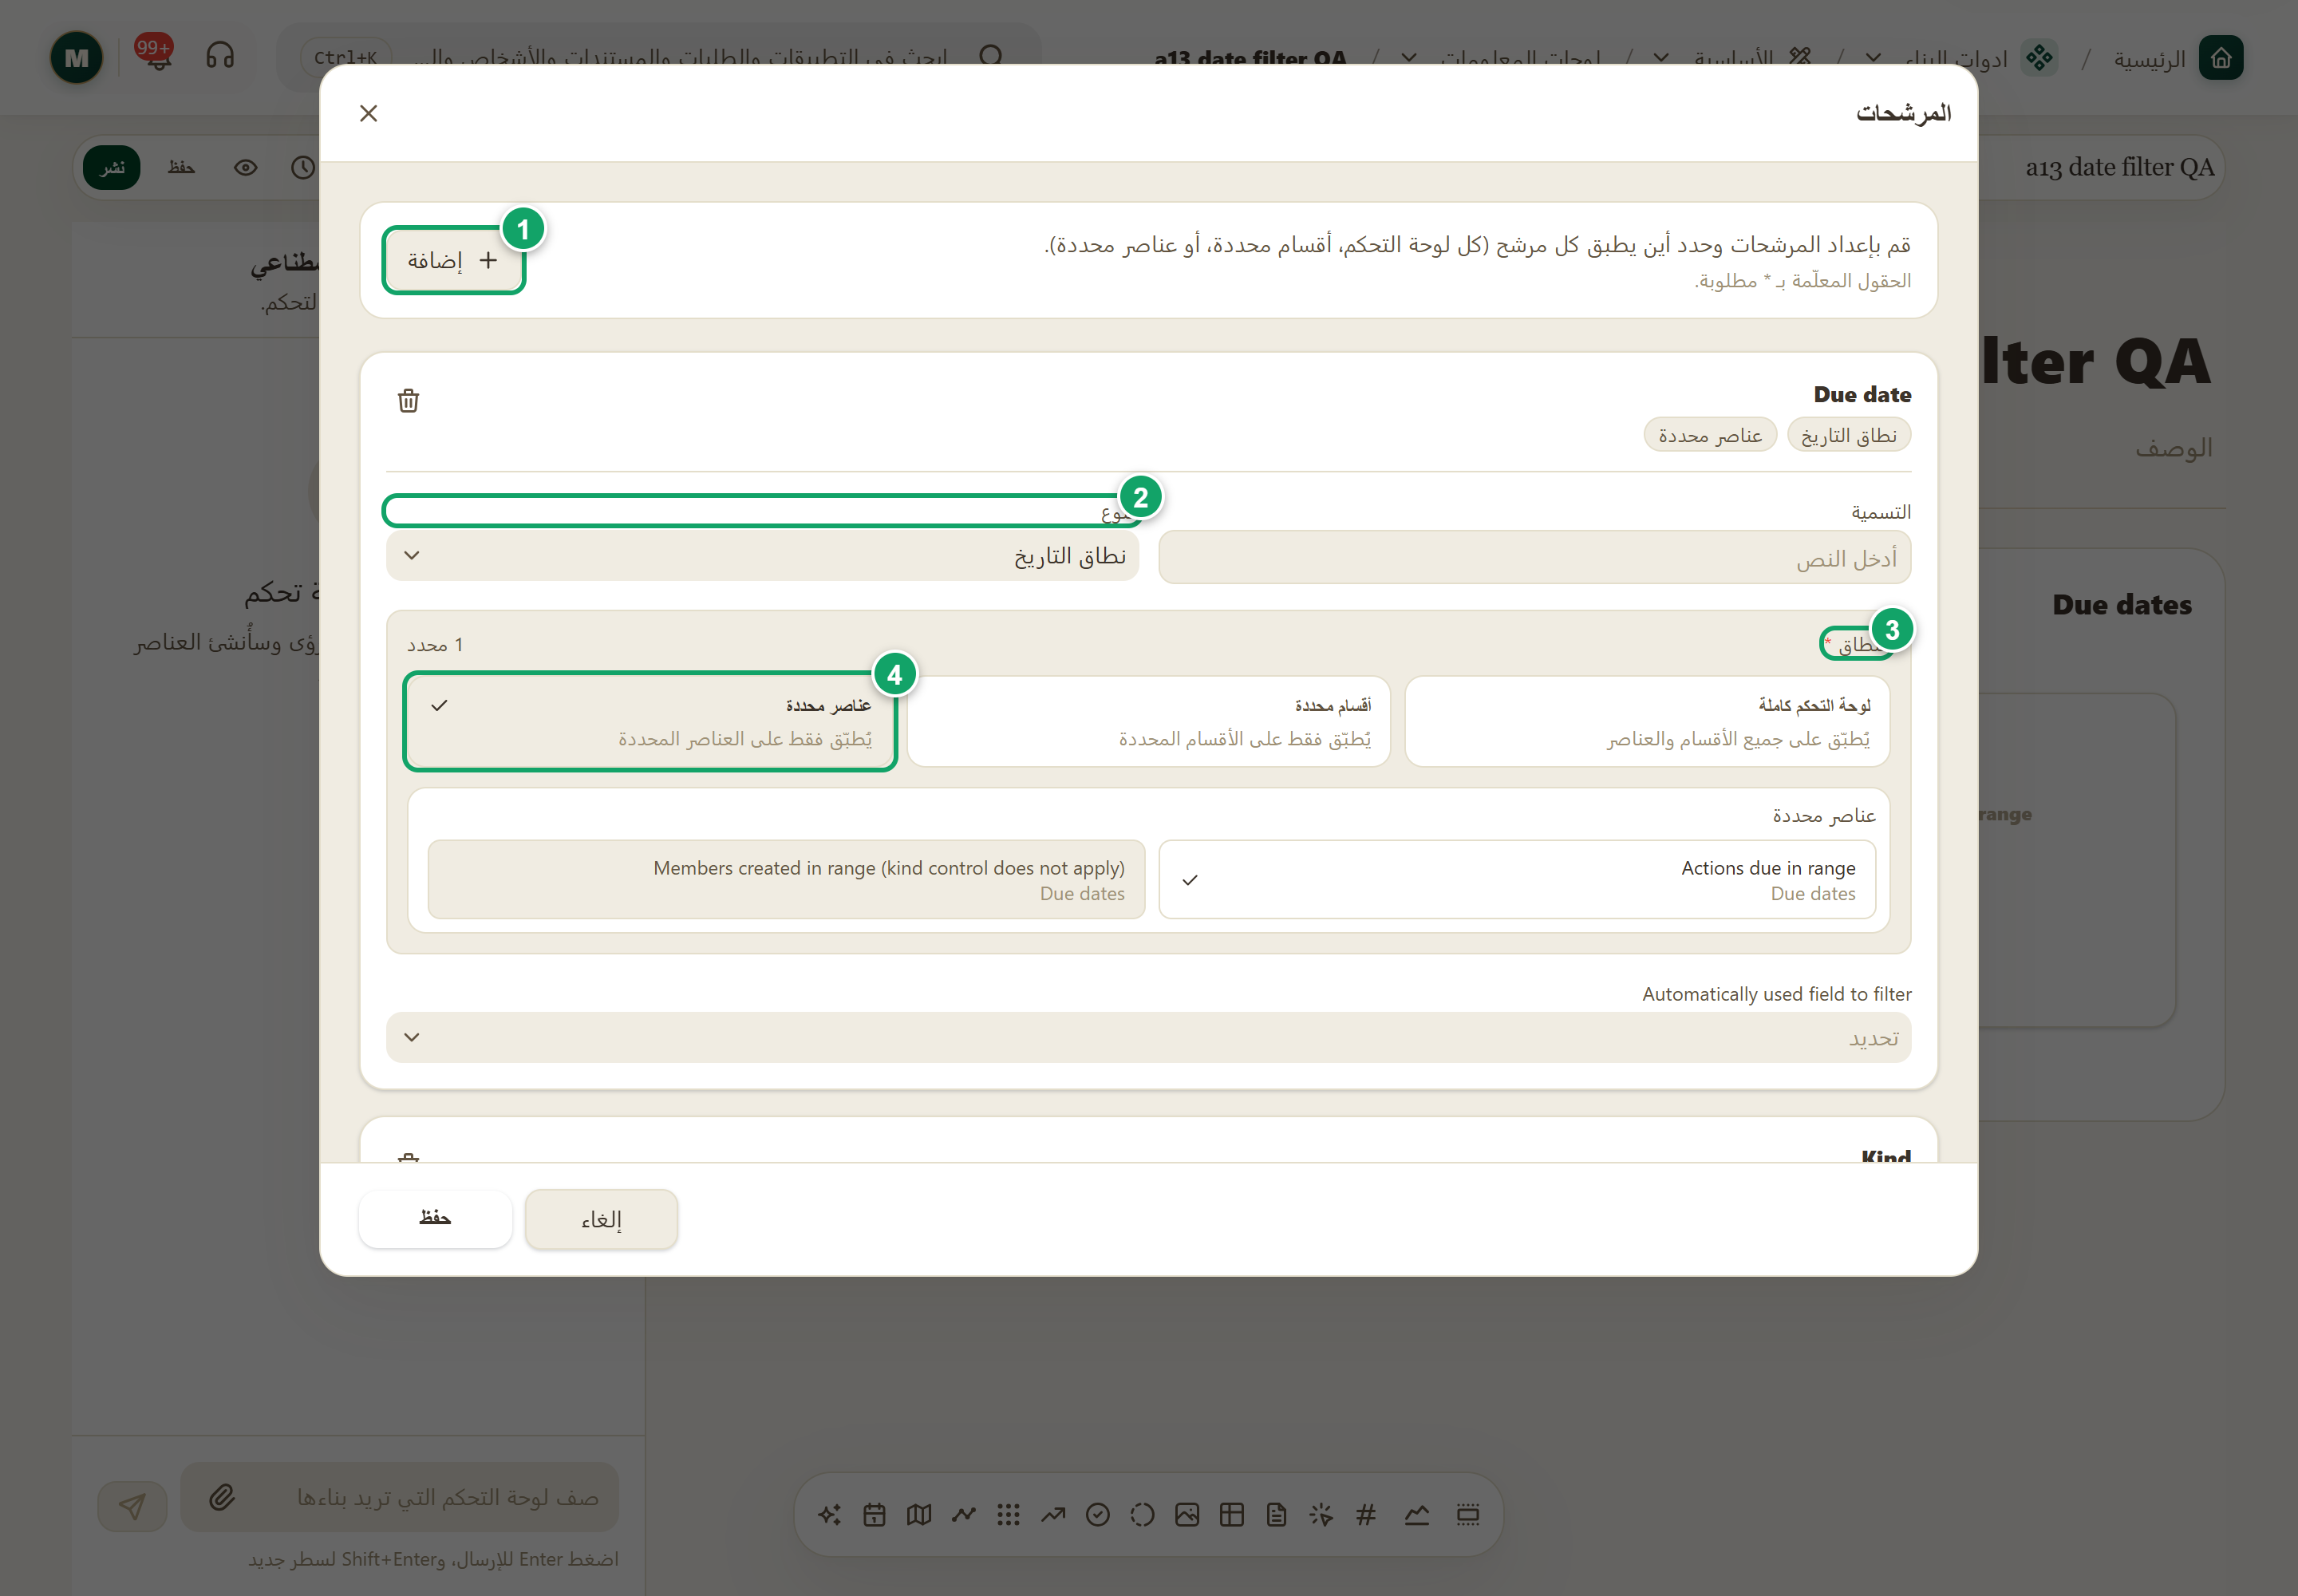
\includegraphics[width=0.95\linewidth,height=0.72\textheight,keepaspectratio]{figures/screens/ch06-dash-filters-ar.png}
\caption{نافذة «المرشحات» في المنشئ}
\label{fig:builder-dashboards-filters-screen}
\shotnote{تعرض الصورة مرشح «نطاق التاريخ» في لوحة اختبار، وقد قُصر نطاقه على عنصر واحد من عنصري القسم. ويبيّن ذلك أن المرشح لا يغيّر إلا العناصر التي يشملها نطاقه، ولو ظهرت كلها في القسم نفسه. ① «إضافة»: يضيف مرشحاً جديداً. ② «النوع»: «نطاق التاريخ» أو «محدد» أو «اختر الحقل». ③ «النطاق»: أين يُطبَّق المرشح. ④ «عناصر محددة»: يطبّقه على العناصر التي تختارها تحته.}
\end{figure}

\begin{table}[H]
\centering
\caption{إعدادات المرشح}
\label{tab:builder-dashboards-filters-fields}
\begin{tabularx}{\linewidth}{R{3.6cm} Y}
\rcHeaderRow
\thh{الإعداد} & \thh{المعنى}\\
«نطاق التاريخ» & تختار حقل التاريخ أو حقوله في كل نوع سجلات، فيقصر المرشح السجلات على الفترة التي يختارها المشاهد.\\
«محدد» & تختار نوع السجلات و«التسمية» و«القيمة الافتراضية (اختياري)»، ويمكن جعله «مطلوب». وتستخدم العناصر قيمته في مرشحاتها عبر معرّف المحدد.\\
«اختر الحقل» & يطابق «الحقل المستهدف» مع خيار يختاره المشاهد. وتأتي الخيارات من «خيارات يدوية» تكتبها، أو «من حقل كيان» من نوع اختيار.\\
«النطاق» & يطبّق المرشح على اللوحة كلها، أو على «أقسام محددة»، أو على «عناصر محددة».\\
\end{tabularx}
\end{table}

\begin{figure}[H]
\centering
\begin{tikzpicture}[node distance=0.5cm]
\node[stepBox] (a) {\RL{اختيار نوع المرشح}};
\node[stepBox,below=of a] (b) {\RL{الحقول أو نوع السجلات}};
\node[stepBox,below=of b] (c) {\RL{تحديد النطاق}};
\node[stepBox,below=of c] (d) {\RL{تجربة المرشح في المعاينة}};
\draw[flowsTo] (a) -- (b);
\draw[flowsTo] (b) -- (c);
\draw[flowsTo] (c) -- (d);
\end{tikzpicture}
\rclegend
\caption{إضافة مرشح للمشاهد}
\label{fig:builder-dashboards-filters-flow}
\shotnote{يضع المخطط النطاق بعد الحقول، لأن المرشح لا يؤثر إلا في العناصر التي تقرأ الحقل الذي ربطته به. ولذلك تأتي التجربة في المعاينة أخيراً، لترى أي العناصر تغيّرت فعلاً عند اختيار فترة أو سجل.}
\end{figure}

\subsection{خطوات العمل والتحقق}
\begin{enumerate}
\item في المنشئ اضغط «المرشحات»، وأضف مرشحاً واختر نوعه.
\item لمرشح «نطاق التاريخ» اختر حقول التاريخ، ولمرشح «محدد» اختر نوع السجلات واكتب «التسمية».
\item اختر «النطاق»: اللوحة كلها، أو «أقسام محددة»، أو «عناصر محددة» ثم حدد الأقسام أو العناصر.
\item اضغط «حفظ»، ثم «معاينة»، وغيّر قيمة المرشح وراقب العناصر.
\end{enumerate}

\textbf{تحقق ومعالجة المشكلة:} يجب أن تتغير أرقام العناصر المشمولة عند تغيير المرشح، وأن يعيدها «مسح الكل» إلى حالها. فإذا رفضت النافذة الحفظ، فأكمل الحقول المميزة، مثل «يرجى اختيار قسم واحد على الأقل.». وإذا لم يتأثر عنصر، فراجع نطاق المرشح والحقل الذي يقرؤه العنصر.

\clearpage
\section{منشئ اللوحة بالذكاء الاصطناعي}
\label{sec:builder-feature-dashboards-ai-builder}

يتيح المنشئ لوحة جانبية تصف فيها اللوحة التي تريدها بكلماتك، فيطرح الذكاء الاصطناعي أسئلة توضيحية ثم يقترح عناصر ومرشحات. ولا يتغير شيء في اللوحة حتى تراجع المقترح وتطبّقه، ثم تبقى النتيجة مسودة تعدّلها وتنشرها كأي لوحة.

\textbf{المسار ومن يستخدمه:} منشئ اللوحة ← اللوحة الجانبية «منشئ لوحات التحكم بالذكاء الاصطناعي»، ويُظهرها الزر الذي يحمل الاسم نفسه أو يخفيها. يستخدمها من يبني اللوحة ويريد بداية سريعة.

\begin{rcnote}[مثال: شركة الأفق]
يكتب مسؤول النظام: «أريد عدد طلبات الزيارة المنتظرة، والطلبات حسب الحالة والفرع، وتقويماً بالمواعيد». فيجيب عن سؤال حول حقل التاريخ، ثم يضغط «تطبيق المقترح» ويراجع العناصر قبل النشر.
\end{rcnote}

\begin{figure}[H]
\centering
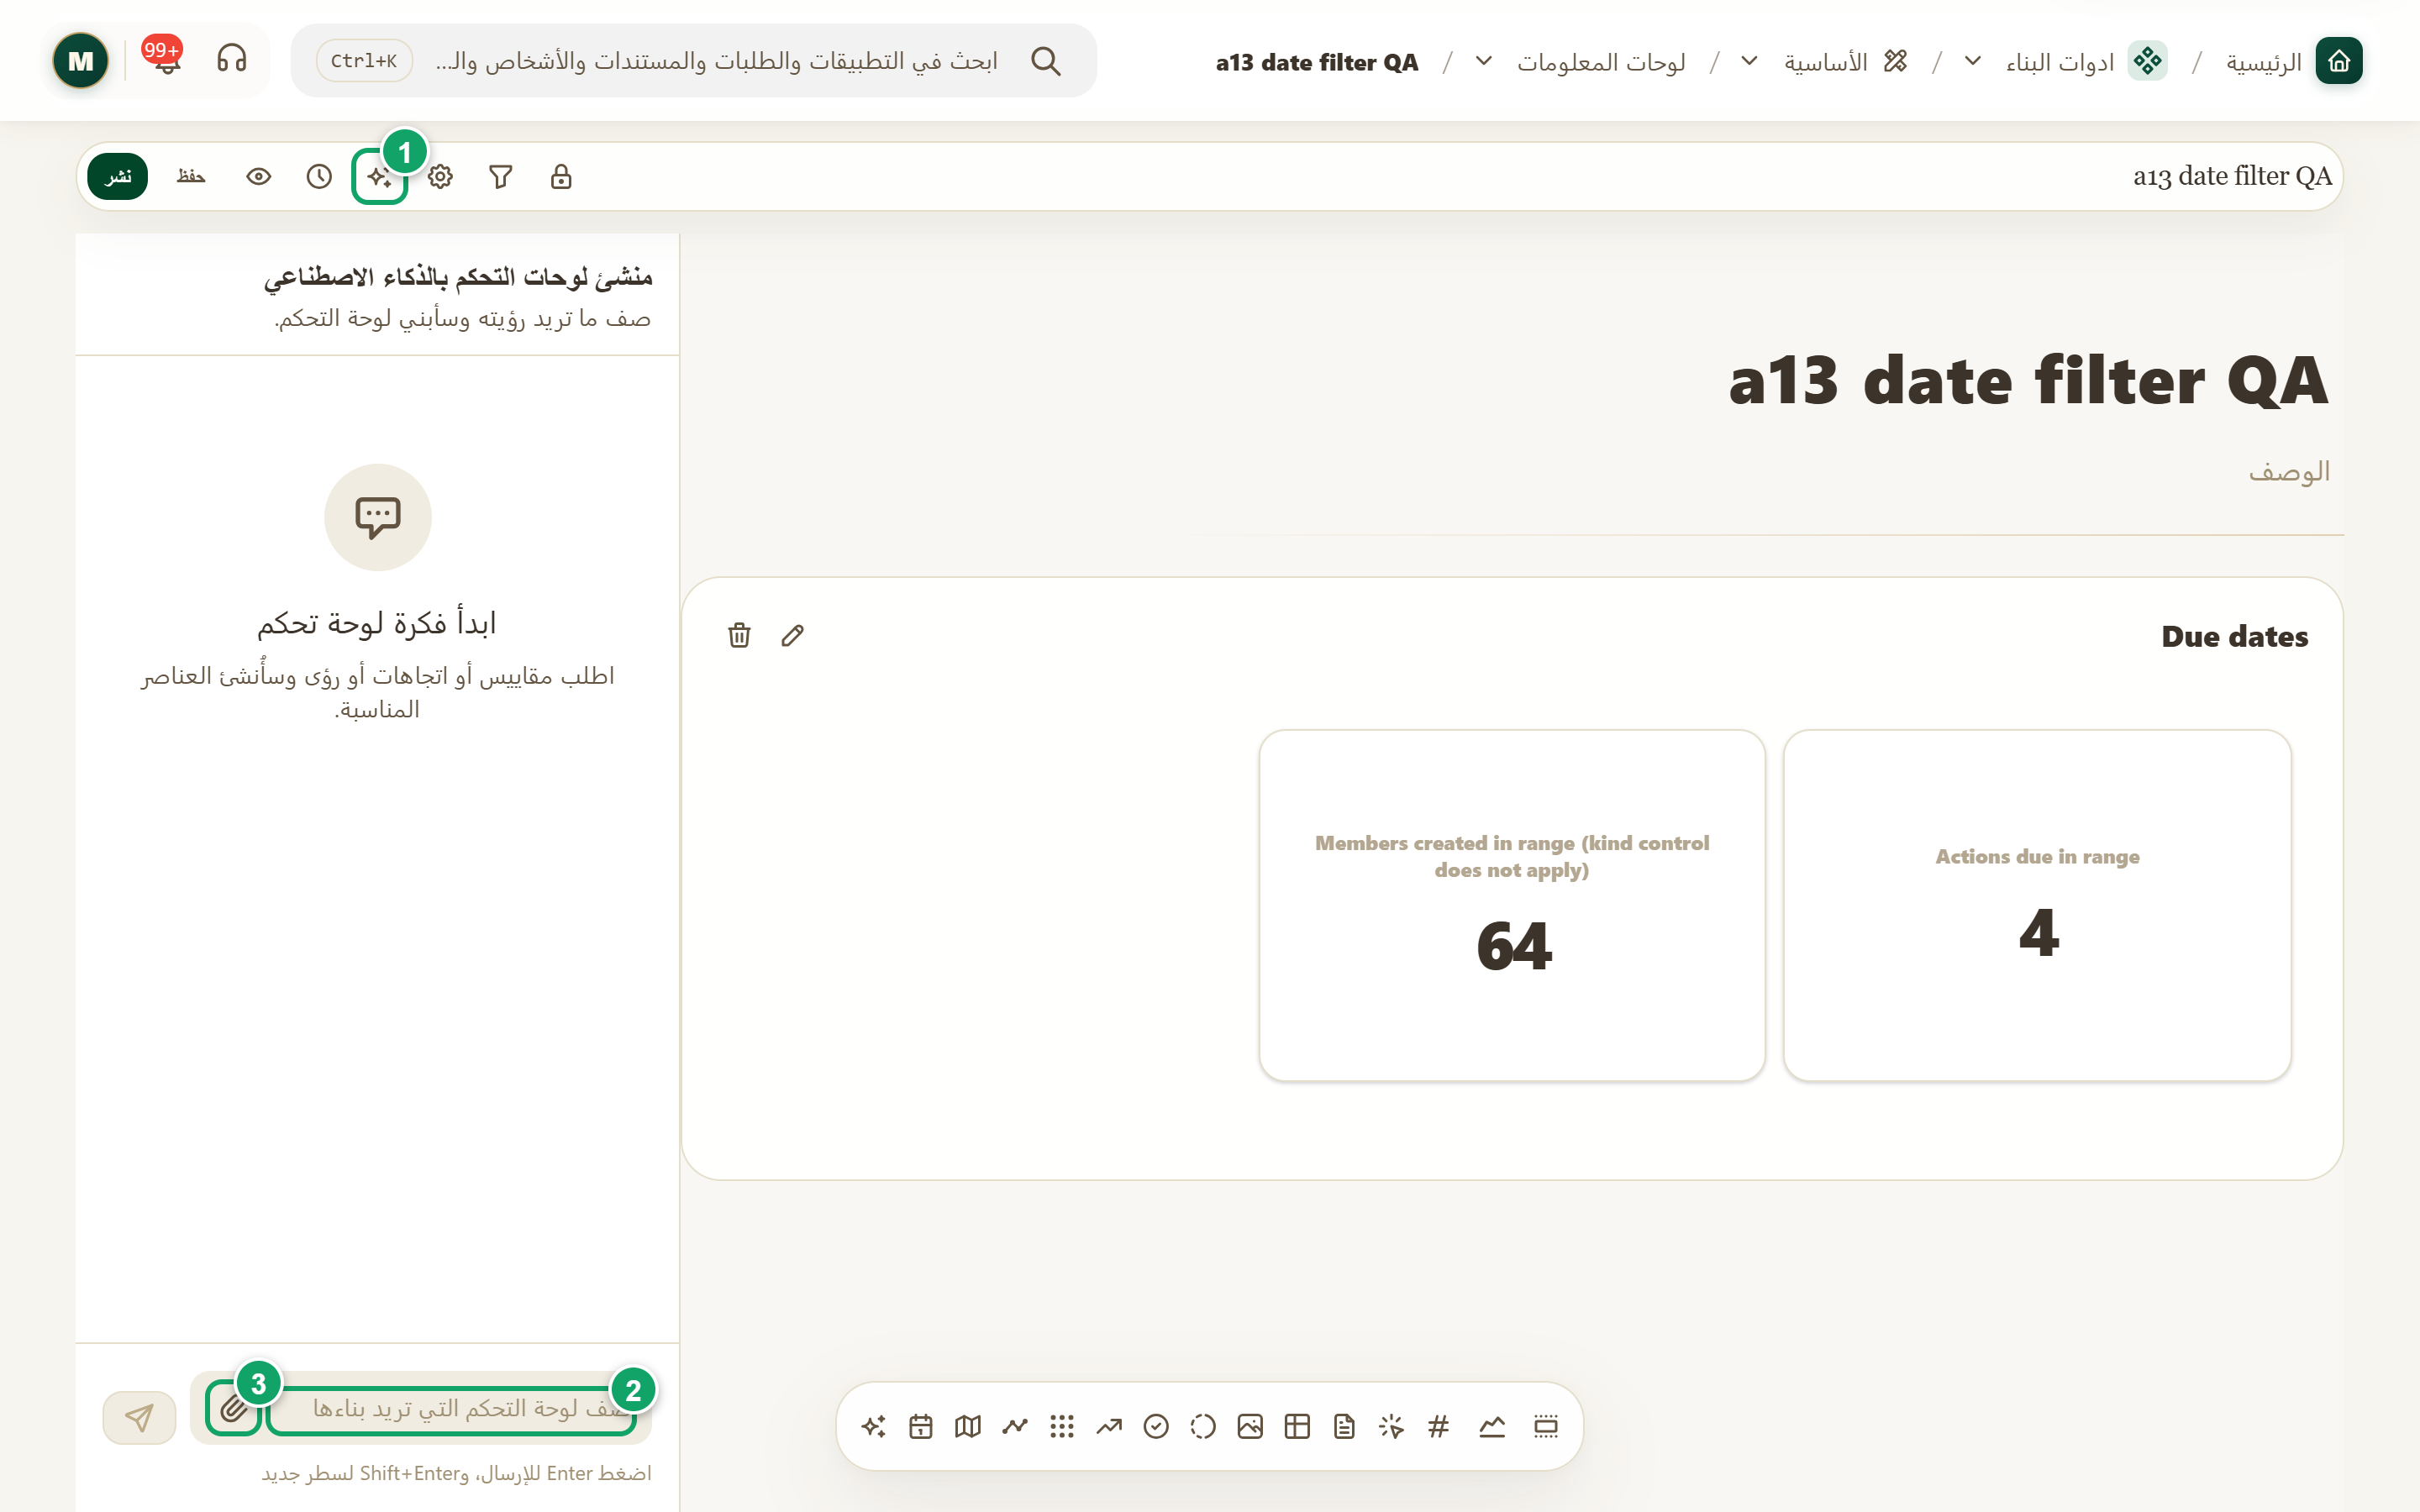
\includegraphics[width=0.95\linewidth,height=0.72\textheight,keepaspectratio]{figures/screens/ch06-dash-ai-builder-ar.png}
\caption{اللوحة الجانبية «منشئ لوحات التحكم بالذكاء الاصطناعي» قبل بدء المحادثة}
\label{fig:builder-dashboards-ai-builder-screen}
\shotnote{تعرض الصورة اللوحة الجانبية ظاهرة في منشئ لوحة اختبار، ولم تبدأ فيها محادثة بعد. ولا يتغير شيء في اللوحة أثناء المحادثة، فالمقترح لا يدخل المسودة إلا عند تطبيقه. ① «منشئ لوحات التحكم بالذكاء الاصطناعي»: يُظهر اللوحة الجانبية أو يخفيها. ② «صف لوحة التحكم التي تريد بناءها»: تكتب فيه طلبك ثم تضغط \en{Enter}. ③ «إرفاق ملف»: يرفق ملفاً يوضح الطلب.}
\end{figure}

\begin{table}[H]
\centering
\caption{مراحل المحادثة}
\label{tab:builder-dashboards-ai-builder-steps}
\begin{tabularx}{\linewidth}{R{3.6cm} Y}
\rcHeaderRow
\thh{المرحلة} & \thh{ما يحدث}\\
الطلب & تكتب في «صف لوحة التحكم التي تريد بناءها» ما تريد رؤيته، ويمكنك «إرفاق ملف» يوضح طلبك.\\
الأسئلة & قد تظهر «يرجى الإجابة على هذه الأسئلة»، فتجيب ثم تضغط «إرسال الإجابات».\\
المقترح & يعرض «ملخص المقترح» عدد العناصر التي يضيفها أو يحدّثها أو يحذفها، وتغييرات المحددات إن وجدت.\\
التطبيق & يضع «تطبيق المقترح» التغييرات في المسودة، وتقبل تغييرات المحددات أو ترفضها بزري «قبول» و«رفض».\\
\end{tabularx}
\end{table}

\begin{figure}[H]
\centering
\begin{tikzpicture}[node distance=0.5cm]
\node[stepBox] (a) {\RL{وصف اللوحة المطلوبة}};
\node[stepBox,below=of a] (b) {\RL{الإجابة عن الأسئلة}};
\node[stepBox,below=of b] (c) {\RL{مراجعة ملخص المقترح}};
\node[stepBox,below=of c] (d) {\RL{تطبيق المقترح}};
\node[stepBox,below=of d] (e) {\RL{مراجعة العناصر ثم النشر}};
\draw[flowsTo] (a) -- (b);
\draw[flowsTo] (b) -- (c);
\draw[flowsTo] (c) -- (d);
\draw[flowsTo] (d) -- (e);
\end{tikzpicture}
\rclegend
\caption{بناء لوحة بمساعدة الذكاء الاصطناعي}
\label{fig:builder-dashboards-ai-builder-flow}
\shotnote{يفصل المخطط بين تطبيق المقترح ونشره، لأن التطبيق يغيّر المسودة فقط. فتراجع كل عنصر ومصدره ومستوى الوصول فيه بعد التطبيق، ثم تنشر عندما تتأكد أن الأرقام صحيحة.}
\end{figure}

\subsection{خطوات العمل والتحقق}
\begin{enumerate}
\item في المنشئ، إذا لم تظهر اللوحة الجانبية، فاضغط «منشئ لوحات التحكم بالذكاء الاصطناعي».
\item اكتب ما تريد رؤيته مع نوع السجلات والفترة، ثم اضغط \en{Enter} للإرسال.
\item أجب عن الأسئلة إن ظهرت واضغط «إرسال الإجابات»، ثم راجع «ملخص المقترح».
\item اضغط «تطبيق المقترح»، ثم افتح كل عنصر وراجع مصدر بياناته و«مستوى الوصول» قبل «حفظ» و«نشر».
\end{enumerate}

\textbf{تحقق ومعالجة المشكلة:} يجب أن يتحول الزر إلى «تم التطبيق» وأن تظهر العناصر في المنشئ. فإذا لم يطابق المقترح ما أردت، فاكتب طلباً أدق بدلاً من تطبيقه. وإذا ظهر «خطأ في العنصر» في عنصر مقترح، فاستخدم «إرسال الخطأ إلى الذكاء الاصطناعي» ليصححه، أو اضبط العنصر يدوياً.

\clearpage
\section{المعاينة والنشر والإصدارات}
\label{sec:builder-feature-dashboards-publish}

يحفظ المنشئ عملك مسودةً لا يراها المشاهدون. وتعرض «معاينة» اللوحة كما ستظهر لهم، ثم يُنشئ «نشر» إصداراً جديداً يحل محل الإصدار المنشور. ويحتفظ «سجل الإصدارات» بالإصدارات السابقة، فتعود إلى أي منها عند الحاجة.

\textbf{المسار ومن يستخدمه:} منشئ اللوحة ← «معاينة» أو «نشر» أو «الإصدارات». يستخدمها من يملك صلاحية تعديل اللوحة.

\begin{rcnote}[مثال: شركة الأفق]
يعاين مسؤول النظام لوحة «متابعة الزيارات» فيرى أن عدد الطلبات المنتظرة يطابق ما في القائمة، فيضغط «نشر». وبعد أسبوع يحذف عنصراً بالخطأ، فيستعيد الإصدار السابق من «سجل الإصدارات».
\end{rcnote}

\begin{figure}[H]
\centering
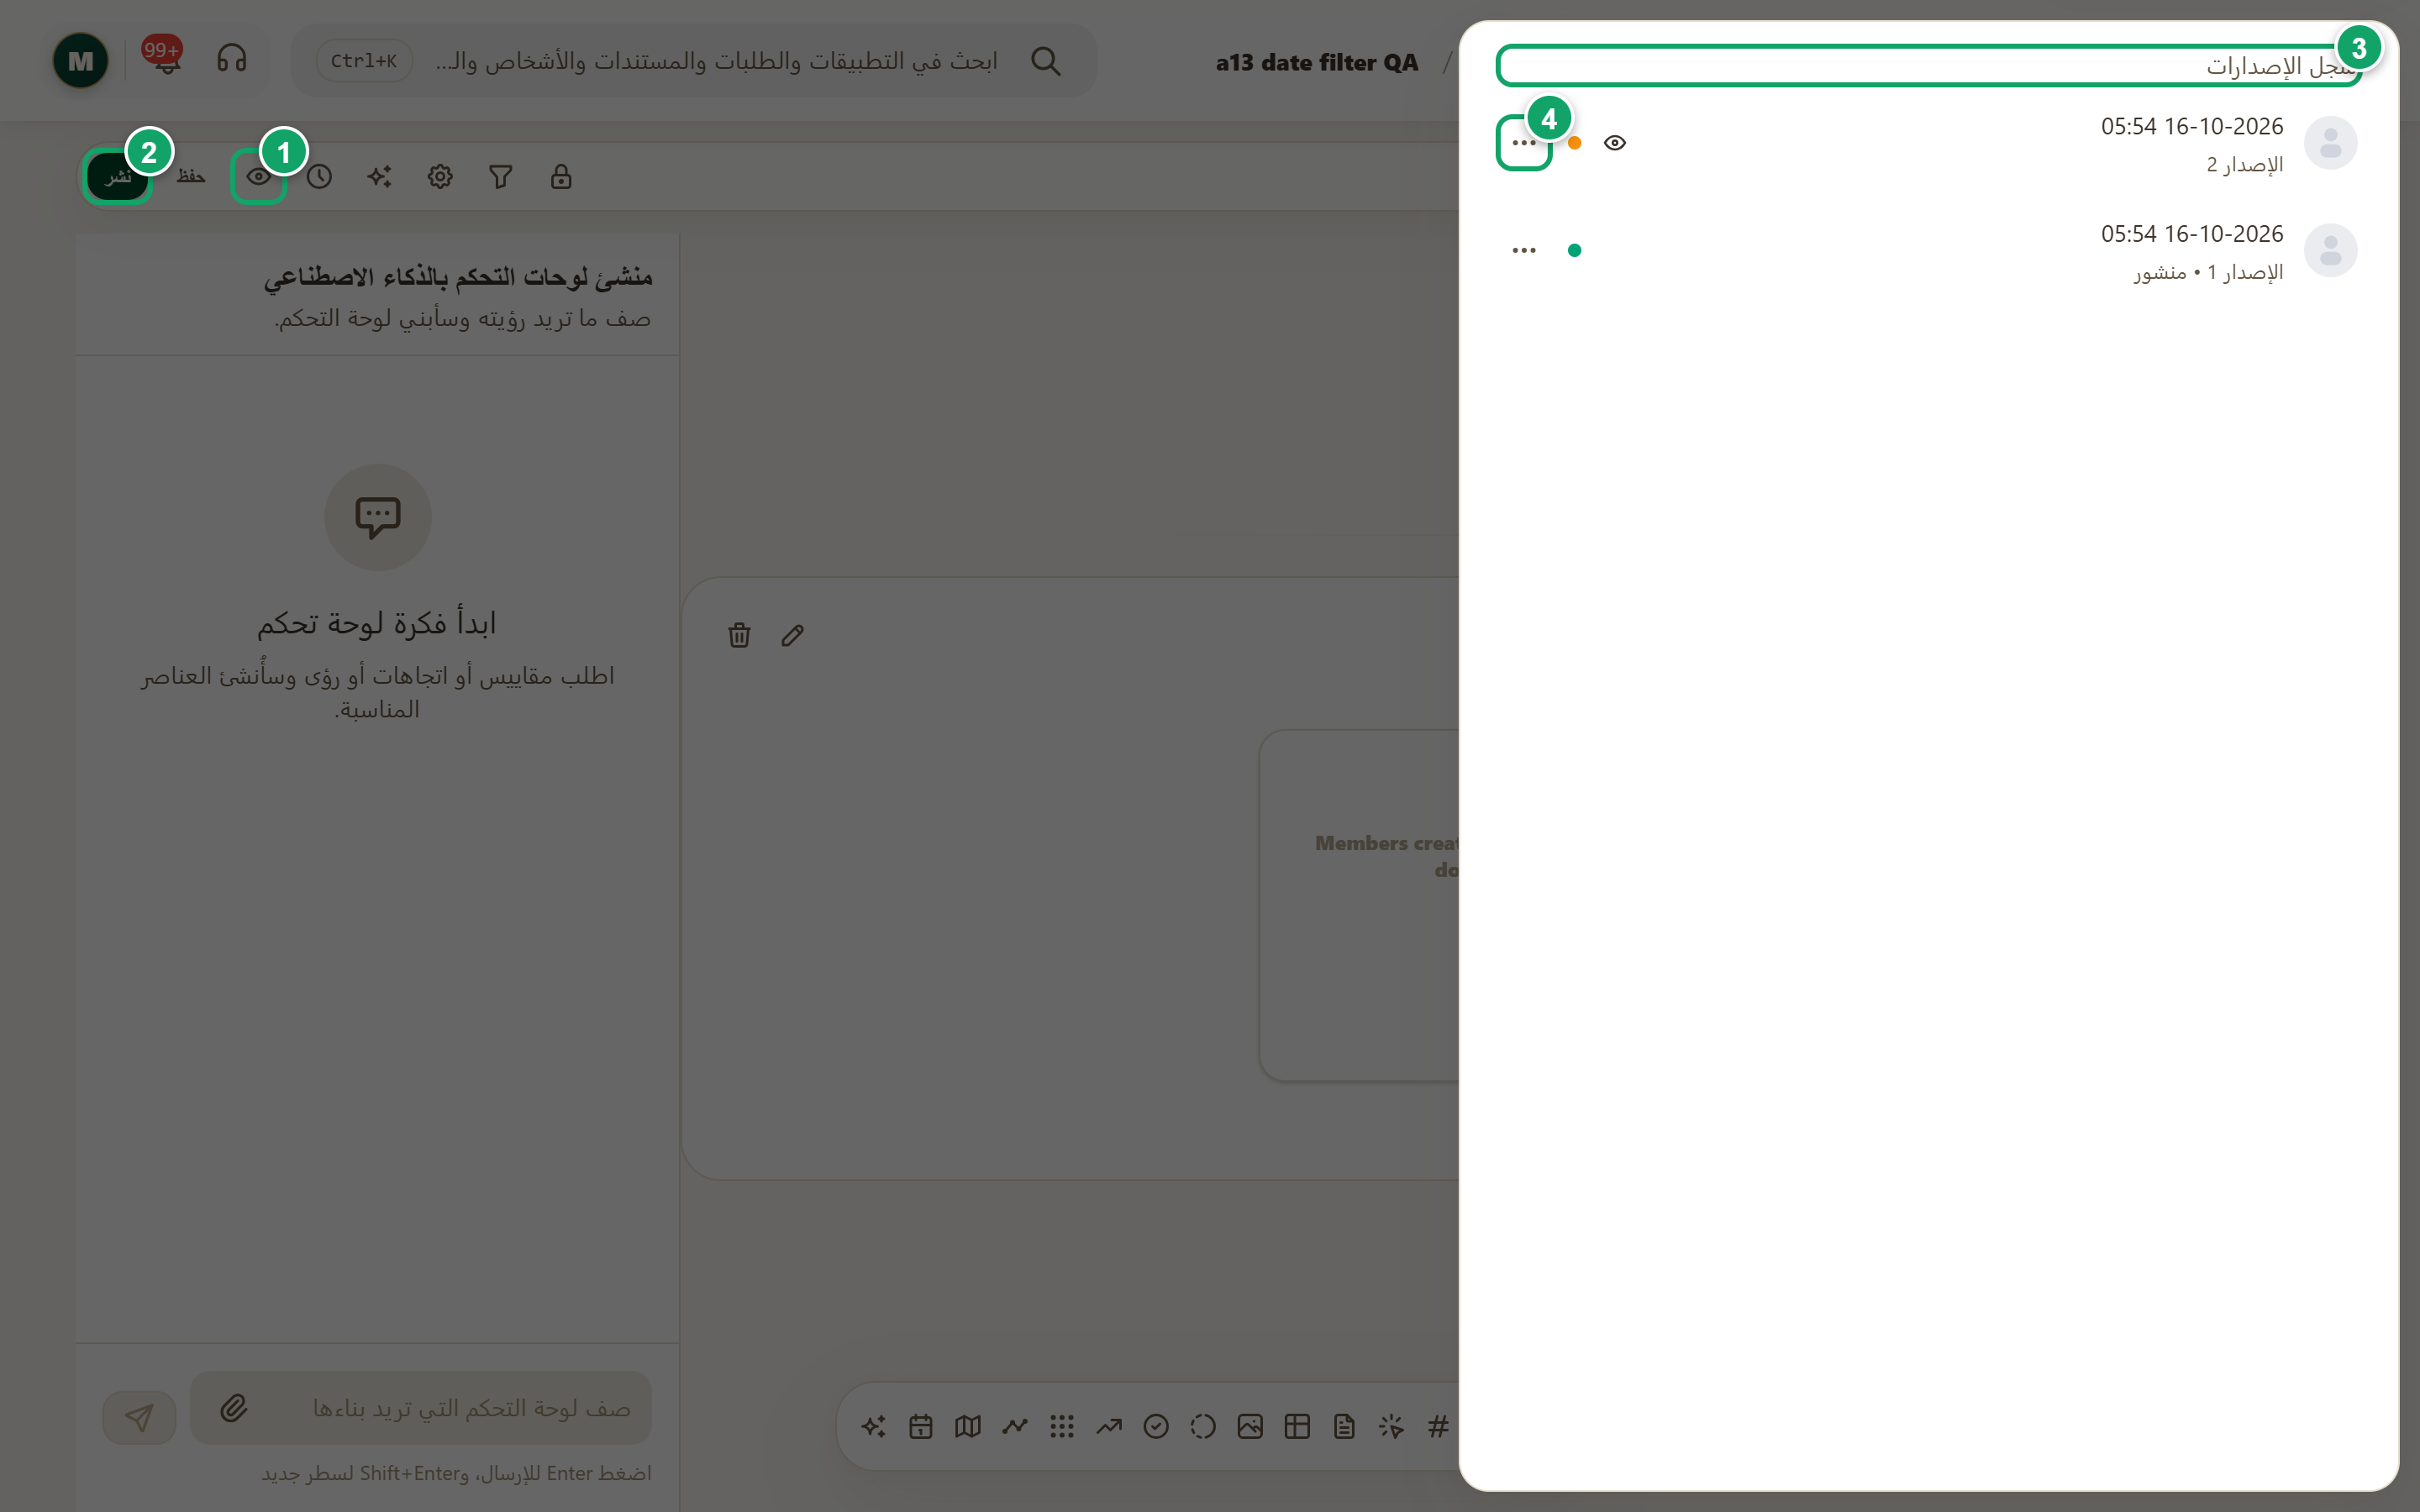
\includegraphics[width=0.95\linewidth,height=0.72\textheight,keepaspectratio]{figures/screens/ch06-dash-versions-ar.png}
\caption{نافذة «سجل الإصدارات» مع زري المعاينة والنشر}
\label{fig:builder-dashboards-publish-screen}
\shotnote{تعرض الصورة سجل إصدارات لوحة اختبار فيه إصداران: الأول منشور بنقطة خضراء، والثاني مسودة أحدث بنقطة برتقالية لم تُنشر بعد. ويبيّن ذلك أن ما يراه المشاهدون هو الإصدار المنشور، لا آخر ما حُفظ في المنشئ. ① «معاينة»: يعرض اللوحة كما يراها المشاهد. ② «نشر»: يحفظ المسودة وينشرها إصداراً جديداً. ③ «سجل الإصدارات»: قائمة الإصدارات بأرقامها وتواريخها. ④ «المزيد من الخيارات»: قائمة الإصدار التي فيها «عرض» و«استعادة».}
\end{figure}

\begin{table}[H]
\centering
\caption{أدوات المعاينة والنشر}
\label{tab:builder-dashboards-publish-tools}
\begin{tabularx}{\linewidth}{R{3.6cm} Y}
\rcHeaderRow
\thh{الأداة} & \thh{ما تفعله}\\
«معاينة» & تعرض اللوحة بالبيانات الحقيقية دون أدوات التعديل، مع شريط «معاينة لوحة المعلومات»، وتعود منها بزر «خروج من المعاينة».\\
«حفظ» & يحفظ المسودة دون أن يغيّر ما يراه المشاهدون.\\
«نشر» & يحفظ ما في المنشئ ثم ينشره إصداراً جديداً، وتظهر رسالة «تم نشر لوحة المعلومات بنجاح».\\
«سجل الإصدارات» & يعرض كل إصدار برقمه وتاريخه، ويُكتب بجانب الإصدار المنشور «منشور» مع نقطة خضراء، وتميّز النقطة البرتقالية المسودة. ومن قائمة الإصدار تختار «عرض»، أو «تعديل كمسودة»، أو «استعادة».\\
\end{tabularx}
\end{table}

\begin{rcwarn}[الاستعادة تستبدل المسودة الحالية]
يستبدل «تعديل كمسودة» و«استعادة» المسودة الحالية بالإصدار الذي اخترته، فتضيع التعديلات غير المنشورة. ولا يرى المشاهدون الإصدار المستعاد حتى تنشره.
\end{rcwarn}

\begin{figure}[H]
\centering
\begin{tikzpicture}[node distance=0.5cm]
\node[stepBox] (a) {\RL{حفظ المسودة}};
\node[stepBox,below=of a] (b) {\RL{معاينة ومقارنة بسجلات معروفة}};
\node[stepBox,below=of b] (c) {\RL{نشر إصدار جديد}};
\node[stepBox,below=of c] (d) {\RL{استعادة إصدار سابق عند الخطأ}};
\draw[flowsTo] (a) -- (b);
\draw[flowsTo] (b) -- (c);
\draw[flowsTo] (c) -- (d);
\end{tikzpicture}
\rclegend
\caption{من المسودة إلى إصدار منشور}
\label{fig:builder-dashboards-publish-flow}
\shotnote{يضع المخطط المقارنة بسجلات معروفة قبل النشر، لأن الرقم الخاطئ في لوحة يقود إلى قرار خاطئ؛ فإذا كنت تعرف أن خمسة طلبات تنتظر، فيجب أن يعرض العنصر خمسة. وتأتي الاستعادة أخيراً بوصفها طريق العودة إذا ظهر خطأ بعد النشر.}
\end{figure}

\subsection{خطوات العمل والتحقق}
\begin{enumerate}
\item اضغط «حفظ»، ثم «معاينة»، وقارن أرقام العناصر بسجلات تعرفها.
\item اضغط «خروج من المعاينة» وصحّح ما يلزم، ثم اضغط «نشر».
\item لاستعادة إصدار، اضغط «الإصدارات»، وافتح قائمة الإصدار واختر «استعادة» ثم أكّد.
\item انشر اللوحة مرة أخرى ليصل الإصدار المستعاد إلى المشاهدين.
\end{enumerate}

\textbf{تحقق ومعالجة المشكلة:} يجب أن يظهر في «سجل الإصدارات» إصدار جديد بحالة «منشور». فإذا ظهرت «فشل نشر لوحة المعلومات. يرجى المحاولة مرة أخرى.»، فاحفظ أولاً ثم أعد النشر. وإذا رأى المشاهدون النسخة القديمة، فتأكد أنك نشرت بعد آخر تعديل.

\clearpage
\section{عرض اللوحة وتصديرها}
\label{sec:builder-feature-dashboards-viewing}

يفتح المشاهد اللوحة المنشورة من التنقل أو من قائمة «لوحات المعلومات»، فيرى الإصدار المنشور بحسب صلاحياته. ويستطيع تغيير المرشحات التي أعدّها صاحب اللوحة، وتصدير بيانات جدول، وتصدير اللوحة كلها تقريراً بصيغة \en{PDF}.

\textbf{المسار ومن يستخدمه:} قسم التطبيق الذي تظهر فيه اللوحة، أو «لوحات المعلومات» ← قائمة البطاقة ← «عرض». يستخدمها كل من مُنح الوصول إلى اللوحة.

\begin{rcnote}[مثال: شركة الأفق]
تفتح سارة الخطيب لوحة «متابعة الزيارات» من «خدمات الفروع»، وتختار فرع حلب في المرشح، ثم تضغط «تصدير PDF» لترفق التقرير بمحضر الاجتماع الشهري.
\end{rcnote}

\begin{figure}[H]
\centering
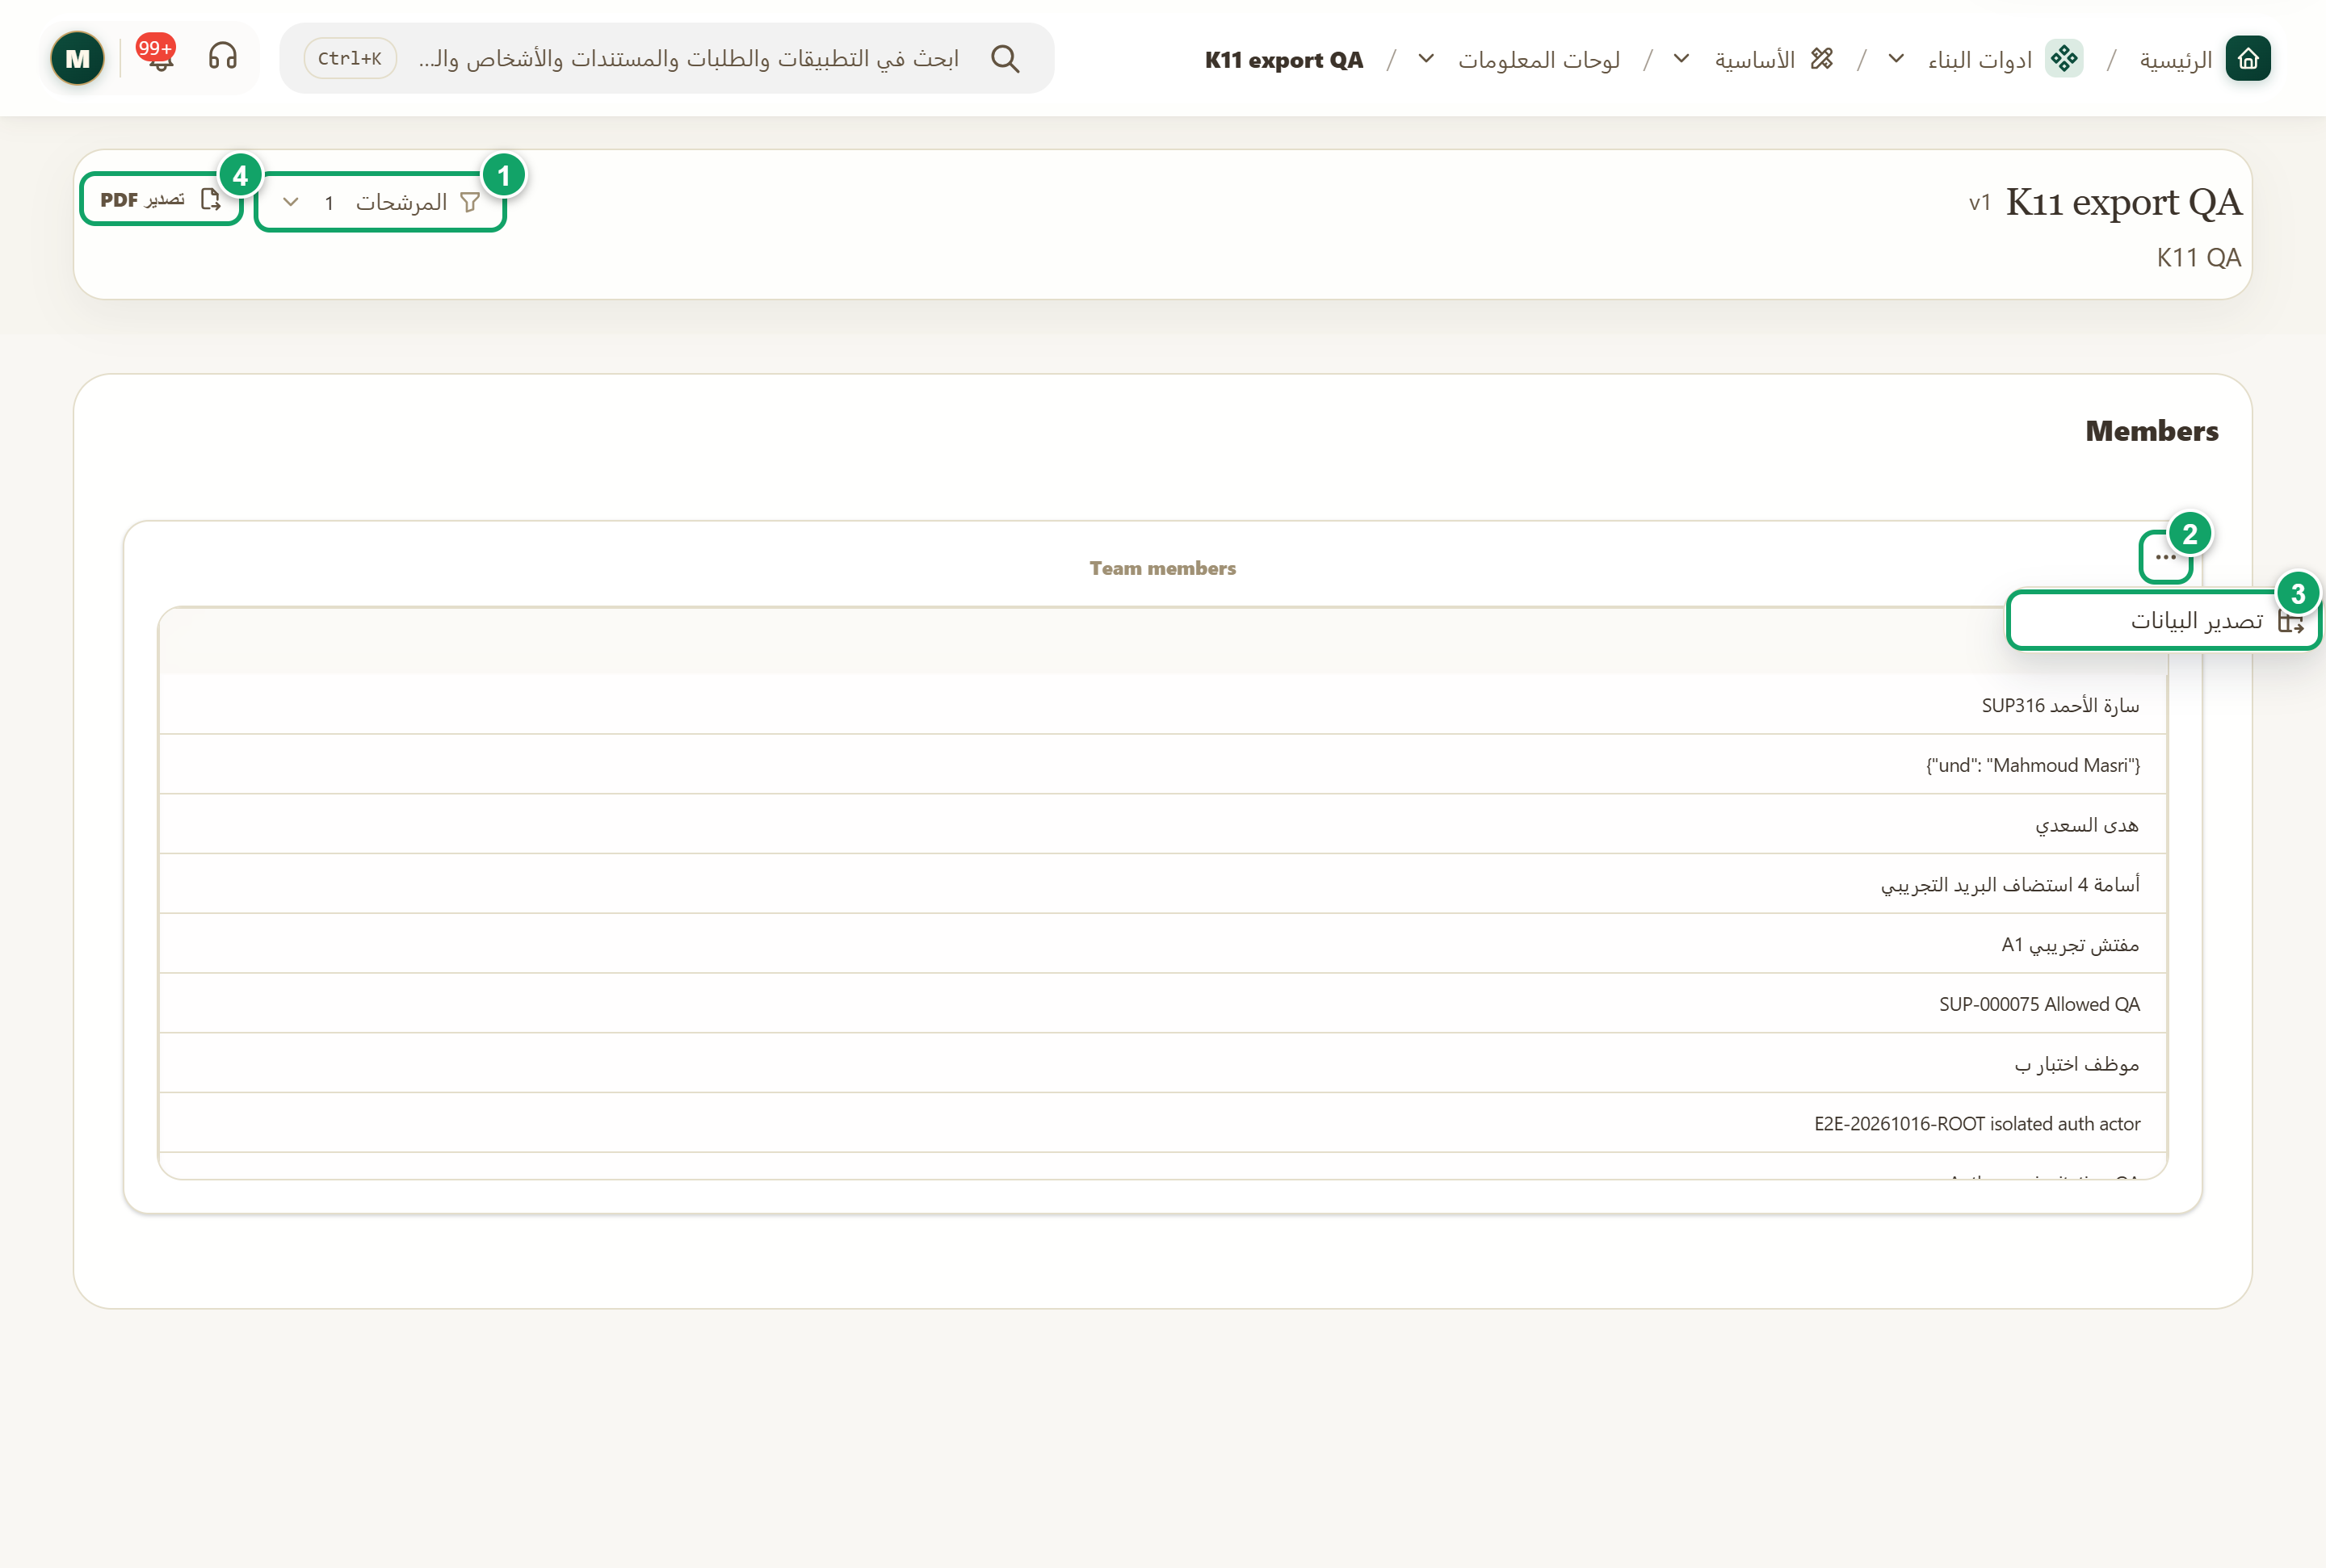
\includegraphics[width=0.95\linewidth,height=0.72\textheight,keepaspectratio]{figures/screens/ch06-dash-view-ar.png}
\caption{لوحة منشورة في وضع العرض مع قائمة «خيارات العنصر»}
\label{fig:builder-dashboards-viewing-screen}
\shotnote{تعرض الصورة لوحة اختبار منشورة فيها جدول كيان، وقد فُتحت قائمة الجدول دون تنفيذ أي تصدير. ويبيّن الرقم بجانب «المرشحات» عدد المرشحات المضبوطة، وهي تنطبق على البيانات المصدّرة أيضاً. ① «المرشحات»: يغيّر بها المشاهد الفترة أو السجل. ② «خيارات العنصر»: زر النقاط في زاوية الجدول. ③ «تصدير البيانات»: يصدّر سجلات الجدول بالمرشحات الحالية. ④ «تصدير PDF»: يجهّز تقريراً من اللوحة كلها.}
\end{figure}

\begin{table}[H]
\centering
\caption{ما يستطيع المشاهد فعله}
\label{tab:builder-dashboards-viewing-actions}
\begin{tabularx}{\linewidth}{R{3.6cm} Y}
\rcHeaderRow
\thh{الإجراء} & \thh{كيف يتم}\\
«المرشحات» & يغيّر المشاهد الفترة أو السجل أو الخيار، فتتغير العناصر المشمولة، ويعيدها «مسح الكل» إلى القيم الافتراضية.\\
«تصدير البيانات» & يظهر في قائمة «خيارات العنصر» لجداول الكيانات لمن يملك صلاحية التصدير، ويُصدّر السجلات بالمرشحات الحالية. وقد يُجهَّز الملف في الخلفية ثم يصل إشعار عند جاهزيته.\\
«تصدير PDF» & يجهّز تقريراً من كل عناصر اللوحة بالمرشحات الحالية، ثم يفتحه في تبويب جديد مع نافذة الطباعة لحفظه بصيغة \en{PDF}.\\
\end{tabularx}
\end{table}

\begin{figure}[H]
\centering
\begin{tikzpicture}[node distance=0.5cm]
\node[stepBox] (a) {\RL{فتح اللوحة المنشورة}};
\node[stepBox,below=of a] (b) {\RL{ضبط المرشحات}};
\node[stepBox,below=of b] (c) {\RL{تصدير البيانات من جدول}};
\node[stepBox,below=of c] (d) {\RL{تصدير PDF للوحة كلها}};
\draw[flowsTo] (a) -- (b);
\draw[flowsTo] (b) -- (c);
\draw[flowsTo] (c) -- (d);
\end{tikzpicture}
\rclegend
\caption{من العرض إلى التقرير}
\label{fig:builder-dashboards-viewing-flow}
\shotnote{يضع المخطط ضبط المرشحات قبل التصدير، لأن الملف والتقرير يحملان الفترة والسجلات المختارة وقت التصدير. وبذلك يطابق ما تشاركه ما رأيته على الشاشة.}
\end{figure}

\subsection{خطوات العمل والتحقق}
\begin{enumerate}
\item افتح اللوحة من قسم التطبيق، أو اختر «عرض» من قائمة بطاقتها.
\item اضبط «المرشحات» على الفترة والسجل المطلوبين.
\item لتصدير جدول، اضغط زر النقاط في زاويته واختر «تصدير البيانات».
\item لتقرير كامل، اضغط «تصدير PDF»، ثم احفظ الملف من نافذة الطباعة.
\end{enumerate}

\textbf{تحقق ومعالجة المشكلة:} يجب أن يعرض التقرير العناصر بالمرشحات التي اخترتها. فإذا ظهرت «يرجى السماح بالنوافذ المنبثقة لفتح تقرير PDF في تبويب جديد.»، فاسمح بها في المتصفح وأعد المحاولة. وإذا لم يظهر «تصدير البيانات»، فأنت لا تملك صلاحية التصدير أو العنصر ليس جدول كيان. وإذا ظهرت «لم يتم نشر لوحة المعلومات بعد»، فاطلب من صاحبها نشرها.

\clearpage
\section{الصفحات}
\label{sec:builder-feature-pages}

الصفحة تضع لوحة معلومات محفوظة من مساحة التحليلات بالذكاء الاصطناعي (\en{DB Genie}) داخل قسم في تطبيق، فتظهر للأعضاء عنصراً في القائمة. وهي الطريقة لمشاركة لوحة صنعتها في «لوحات معلومات الذكاء الاصطناعي» مع الفريق.

\textbf{المسار ومن يستخدمه:} «ادوات البناء» ← «الأساسية» ← «الصفحات». تظهر لمالك المؤسسة ومسؤولها فقط.

\begin{rcnote}[مثال: شركة الأفق]
يصنع مسؤول النظام لوحة تحليل لمدد إنجاز الزيارات في مساحة الذكاء الاصطناعي، ثم ينشرها صفحةً في قسم «الزيارات» داخل «خدمات الفروع» لتراها سارة الخطيب. وتبدأ الصفحة من ①.
\end{rcnote}

\begin{figure}[H]
\centering
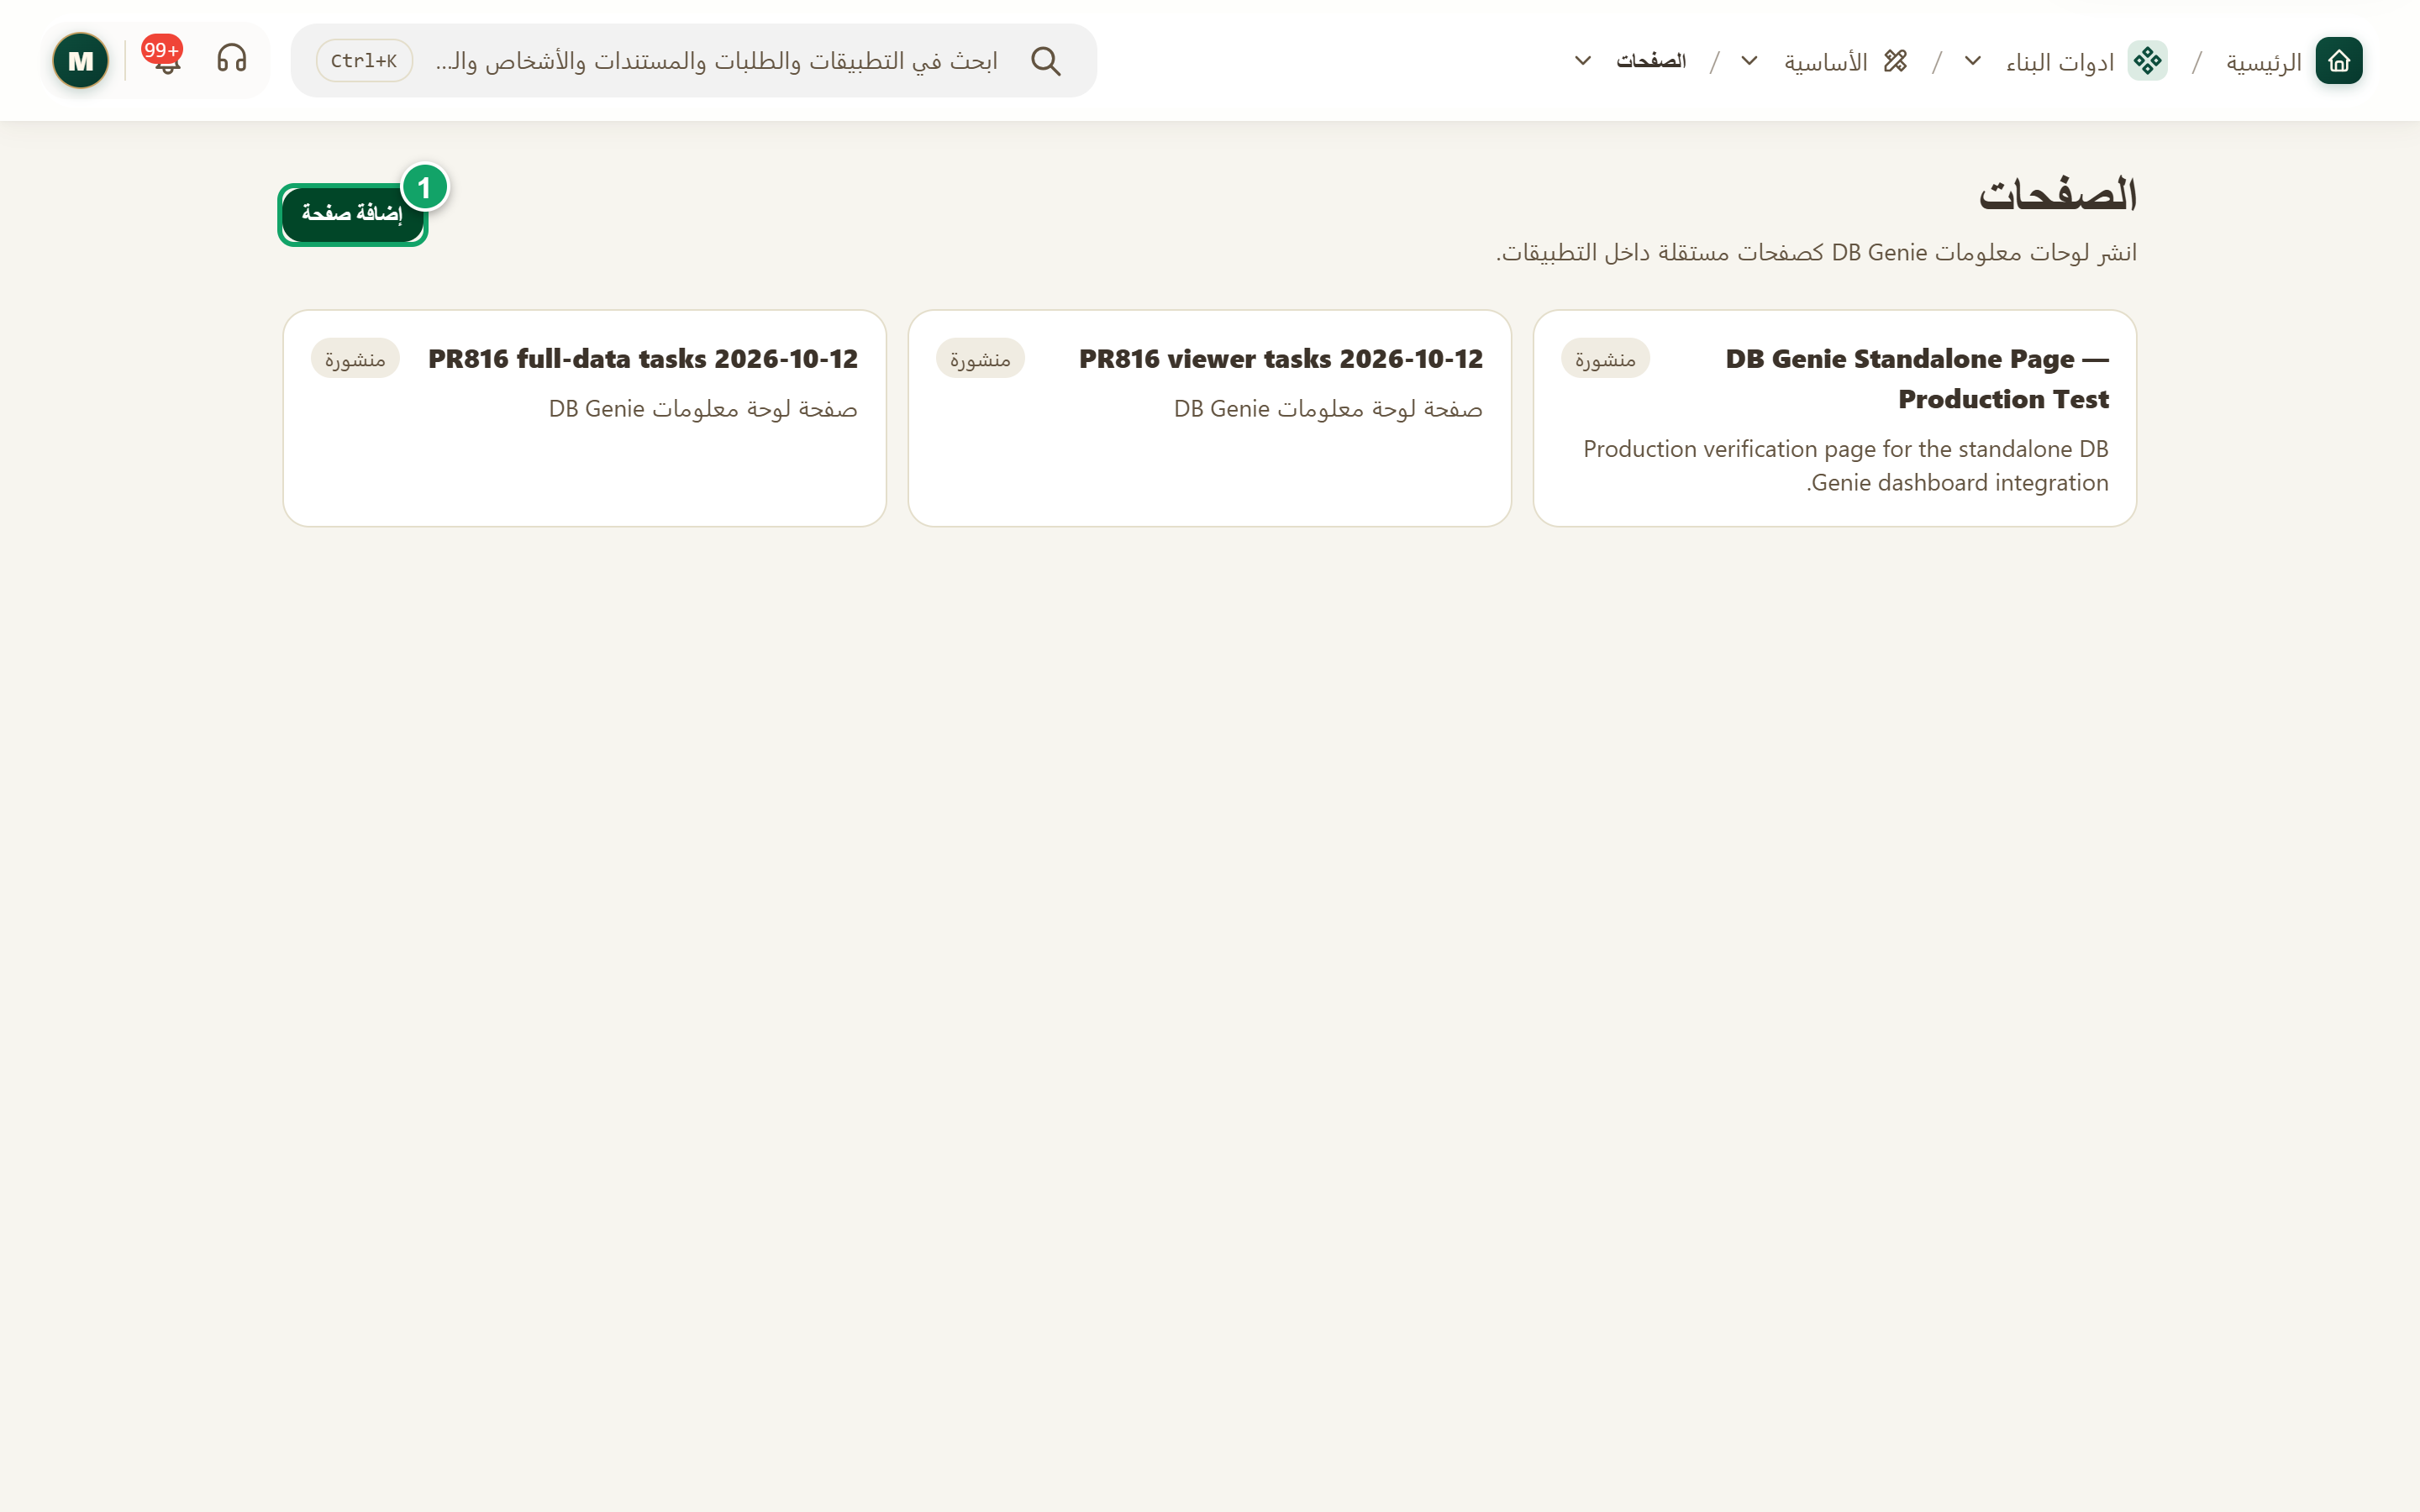
\includegraphics[width=0.95\linewidth,height=0.72\textheight,keepaspectratio]{figures/screens/ch06-pages-ar.png}
\caption{صفحة «الصفحات»}
\label{fig:builder-pages-screen}
\shotnote{تعرض الصفحة الصفحات المستقلة المنشورة في التطبيقات، وهي هنا صفحات اختبار. ① «إضافة صفحة»: تبدأ صفحة جديدة تختار لها اللوحة والتطبيق والقسم.}
\end{figure}


\begin{table}[H]
\centering
\caption{حقول الصفحة}
\label{tab:builder-pages-data}
\begin{tabularx}{\linewidth}{R{3.6cm} Y}
\rcHeaderRow
\thh{الحقل} & \thh{المعنى}\\
العنوان والوصف & اسم الصفحة كما يظهر في القائمة، ووصف قصير.\\
التطبيق والقسم & المكان الذي تظهر فيه الصفحة في التنقل.\\
لوحة معلومات DB Genie & لوحة محفوظة تختارها بزر «اختيار لوحة معلومات».\\
البيانات المعروضة & «بصلاحيات المشاهد» وهو الأكثر أماناً، أو بيانات المؤسسة بحماية، أو بيانات المؤسسة كاملة دون تحقق من نطاق المشاهد.\\
الحالة & «مسودة» أو «منشورة» أو «مؤرشفة». ولا تظهر الصفحة في التنقل إلا وهي منشورة.\\
\end{tabularx}
\end{table}

\begin{figure}[H]
\centering
\begin{tikzpicture}[node distance=0.5cm]
\node[stepBox] (a) {\RL{لوحة في مساحة الذكاء الاصطناعي}};
\node[stepBox,below=of a] (b) {\RL{إضافة صفحة واختيار اللوحة}};
\node[stepBox,below=of b] (c) {\RL{الحالة: منشورة}};
\node[stepBox,below=of c] (d) {\RL{منح صلاحية العرض للأدوار}};
\draw[flowsTo] (a) -- (b);
\draw[flowsTo] (b) -- (c);
\draw[flowsTo] (c) -- (d);
\end{tikzpicture}
\rclegend
\caption{من لوحة خاصة إلى صفحة للفريق}
\label{fig:builder-pages-flow}
\shotnote{يبيّن المخطط أن نشر الصفحة وحده لا يكفي ليراها الأعضاء، بل يحتاج كل دور إلى صلاحية عرض الصفحة في إعدادات الأدوار. وتبقى اللوحة الأصلية كما هي، فحذف الصفحة لا يحذف اللوحة.}
\end{figure}

\subsection{خطوات العمل والتحقق}
\begin{enumerate}
\item احفظ اللوحة في «لوحات معلومات الذكاء الاصطناعي» أولاً.
\item افتح «الصفحات» واضغط «إضافة صفحة»، ثم اكتب العنوان واختر التطبيق والقسم واللوحة.
\item اختر «بصلاحيات المشاهد» في «البيانات المعروضة»، واجعل الحالة «منشورة»، ثم اضغط «حفظ الصفحة».
\item امنح الأدوار المناسبة صلاحية عرض الصفحة من إعدادات الأدوار.
\end{enumerate}

\textbf{تحقق ومعالجة المشكلة:} يجب أن تظهر الصفحة في القسم الذي اخترته لمن يملك صلاحية عرضها. فإذا ظهرت رسالة «العنوان والتطبيق والقسم ولوحة المعلومات مطلوبة»، فأكمل الحقول الأربعة. وإذا لم يرها عضو، فراجع حالتها وصلاحية دوره.

\clearpage
\section{لوحات معلومات الذكاء الاصطناعي}
\label{sec:builder-feature-ai-dashboards}

تفتح هذه الصفحة مساحة التحليلات بالذكاء الاصطناعي (\en{DB Genie})، حيث تصف ما تريد معرفته فتُبنى لك لوحة معلومات من بيانات المؤسسة. وتكون المساحة خاصة بك، ولا تستخدم إلا البيانات التي تستطيع قراءتها. ولمشاركة لوحة مع الفريق، انشرها من صفحة «الصفحات».

\textbf{المسار ومن يستخدمه:} «ادوات البناء» ← «الأساسية» ← «لوحات معلومات الذكاء الاصطناعي». تظهر لمن يتضمن مقعده التحليلات، إذا كان مسؤولاً في المؤسسة أو يملك صلاحية عرض لوحات المعلومات.

\begin{rcnote}[مثال: شركة الأفق]
تطلب سارة الخطيب لوحة توضح عدد الزيارات لكل فرع في كل شهر، فتراجع النتيجة في مساحتها الخاصة قبل أن يقرر مسؤول النظام نشرها صفحةً للفريق. وتطلب سارة اللوحة داخل المساحة ①.
\end{rcnote}

\begin{figure}[H]
\centering
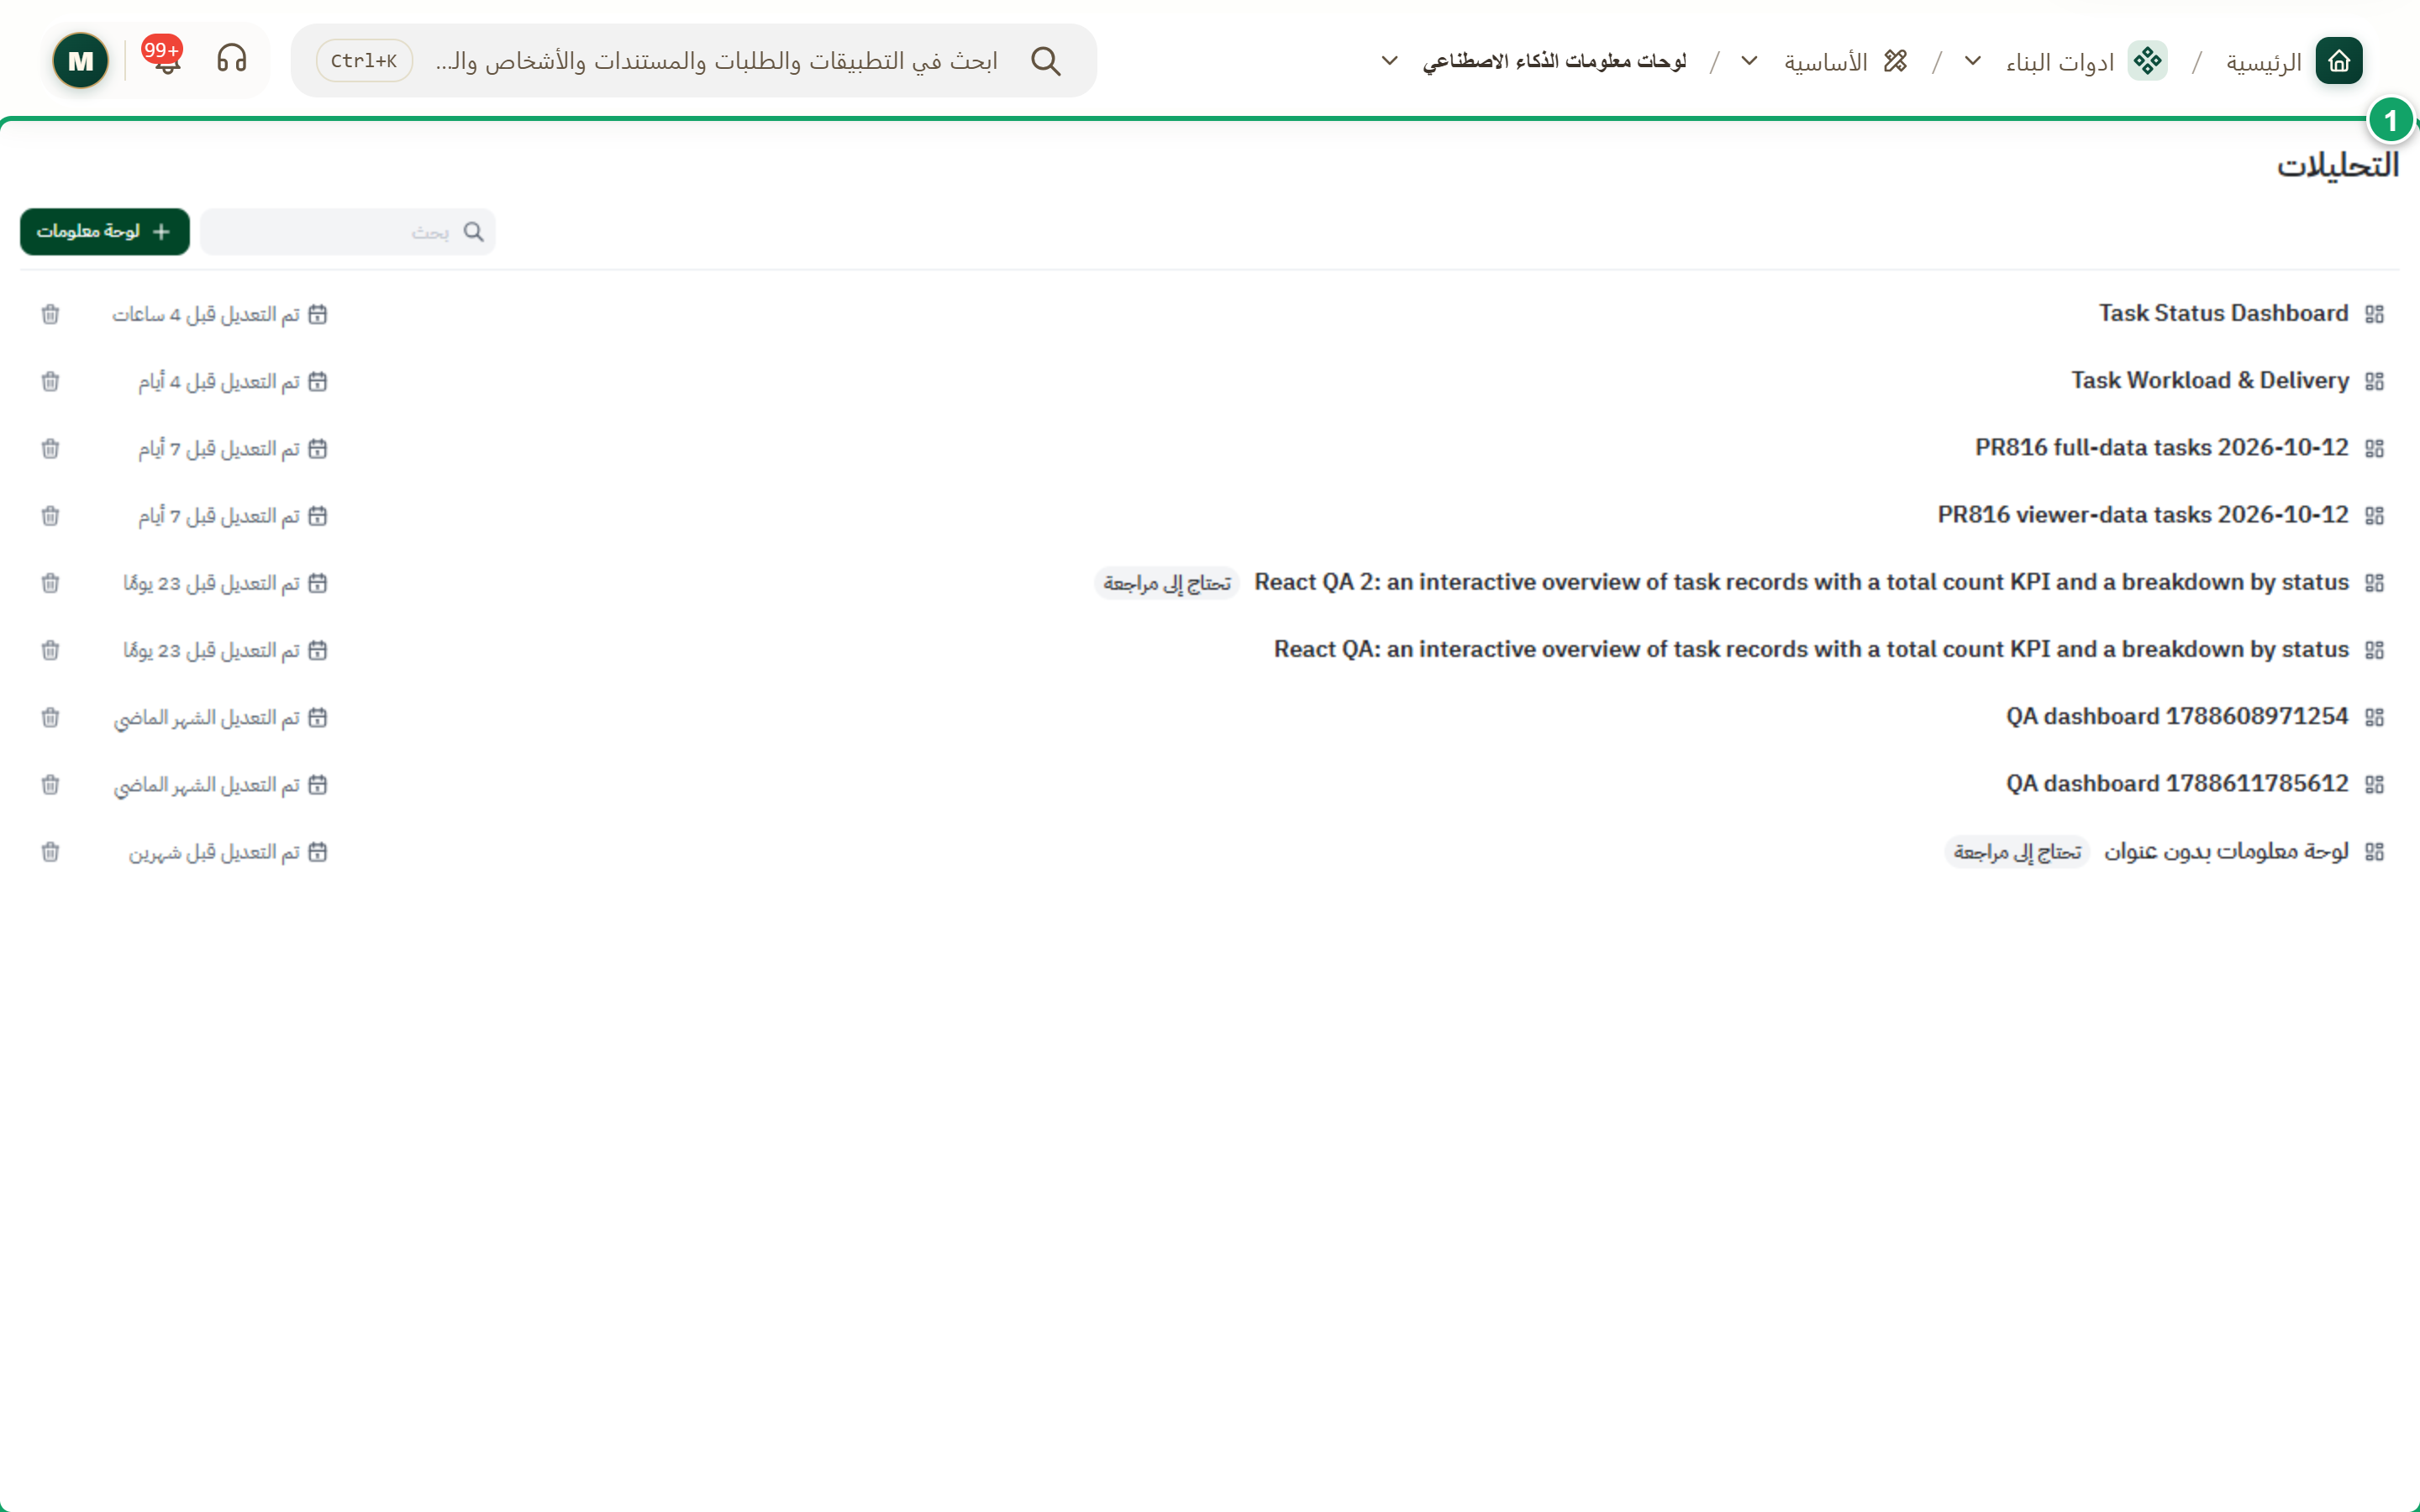
\includegraphics[width=0.95\linewidth,height=0.72\textheight,keepaspectratio]{figures/screens/ch06-ai-dashboards-ar.png}
\caption{مساحة «لوحات معلومات الذكاء الاصطناعي»}
\label{fig:builder-ai-dashboards-screen}
\shotnote{تُفتح مساحة التحليلات داخل كيان، وتعرض لوحات المستخدم الخاصة به. والمحتوى هنا محتوى مؤسسة الاختبار. ① مساحة التحليلات: فيها تُنشأ اللوحات وتُراجَع، ويخدمها نظام التحليلات المضمّن.}
\end{figure}


\begin{table}[H]
\centering
\caption{ما الذي يجب معرفته؟}
\label{tab:builder-ai-dashboards-data}
\begin{tabularx}{\linewidth}{R{3.6cm} Y}
\rcHeaderRow
\thh{الجانب} & \thh{المعنى}\\
مساحة خاصة & اللوحات هنا لك وحدك، وتُحسب من البيانات التي تملك صلاحية قراءتها فقط.\\
بيانات غير متاحة & قد تظهر رسالة بأن بعض البيانات غير متاحة لأن صلاحياتك على أنواع سجلات معينة أوسع من أن تُضمَّن.\\
المشاركة & تُشارك اللوحة بنشرها صفحةً من «الصفحات»، لا من هذه المساحة.\\
\end{tabularx}
\end{table}

\begin{figure}[H]
\centering
\begin{tikzpicture}[node distance=0.5cm]
\node[stepBox] (a) {\RL{وصف ما تريد معرفته}};
\node[stepBox,below=of a] (b) {\RL{مراجعة اللوحة الناتجة}};
\node[stepBox,below=of b] (c) {\RL{نشرها من الصفحات عند الحاجة}};
\draw[flowsTo] (a) -- (b);
\draw[flowsTo] (b) -- (c);
\end{tikzpicture}
\rclegend
\caption{من سؤال إلى لوحة مشتركة}
\label{fig:builder-ai-dashboards-flow}
\shotnote{يضع المخطط المراجعة قبل المشاركة، لأن اللوحة التي يولّدها الذكاء الاصطناعي قد تفهم السؤال على غير ما تقصد. فقارن أرقامها بما تعرفه، ثم شاركها عبر «الصفحات» فقط عندما تثق بها.}
\end{figure}

\subsection{خطوات العمل والتحقق}
\begin{enumerate}
\item افتح «لوحات معلومات الذكاء الاصطناعي»، وانتظر حتى تُحمَّل مساحة التحليلات.
\item أنشئ لوحة جديدة واكتب ما تريد معرفته بوضوح، مع الفترة والحقول المهمة.
\item راجع اللوحة واحفظها، ثم انشرها من «الصفحات» إن أردت أن يراها الفريق.
\end{enumerate}

\textbf{تحقق ومعالجة المشكلة:} يجب أن تُفتح المساحة وتعرض لوحاتك. فإذا ظهرت رسالة «تعذر فتح التحليلات» أو أعادتك الصفحة إلى الرئيسية، فمقعدك لا يتضمن التحليلات أو تنقصك صلاحية عرض لوحات المعلومات؛ فاطلبها من مسؤول المؤسسة.

\clearpage
\section{تقارير الذكاء الاصطناعي}
\label{sec:builder-feature-ai-reports}

تفتح هذه الصفحة مساحة التحليلات نفسها في وضع المحادثة: تسأل بلغتك عن بيانات المؤسسة، فيجيبك الذكاء الاصطناعي بتقرير مكتوب وأرقام. وتناسب الأسئلة السريعة التي لا تحتاج إلى لوحة دائمة، مثل «كم زيارة أُلغيت هذا الشهر ولماذا؟».

\textbf{المسار ومن يستخدمه:} «ادوات البناء» ← «الأساسية» ← «تقارير الذكاء الاصطناعي». شروط ظهورها هي شروط «لوحات معلومات الذكاء الاصطناعي» نفسها.

\begin{rcnote}[مثال: شركة الأفق]
تسأل سارة الخطيب عن الفروع التي تأخرت زياراتها أكثر من أسبوع، فتحصل على تقرير قصير تبني عليه نقاش الاجتماع الشهري. وتطرح سارة سؤالها في المنطقة ①.
\end{rcnote}

\begin{figure}[H]
\centering
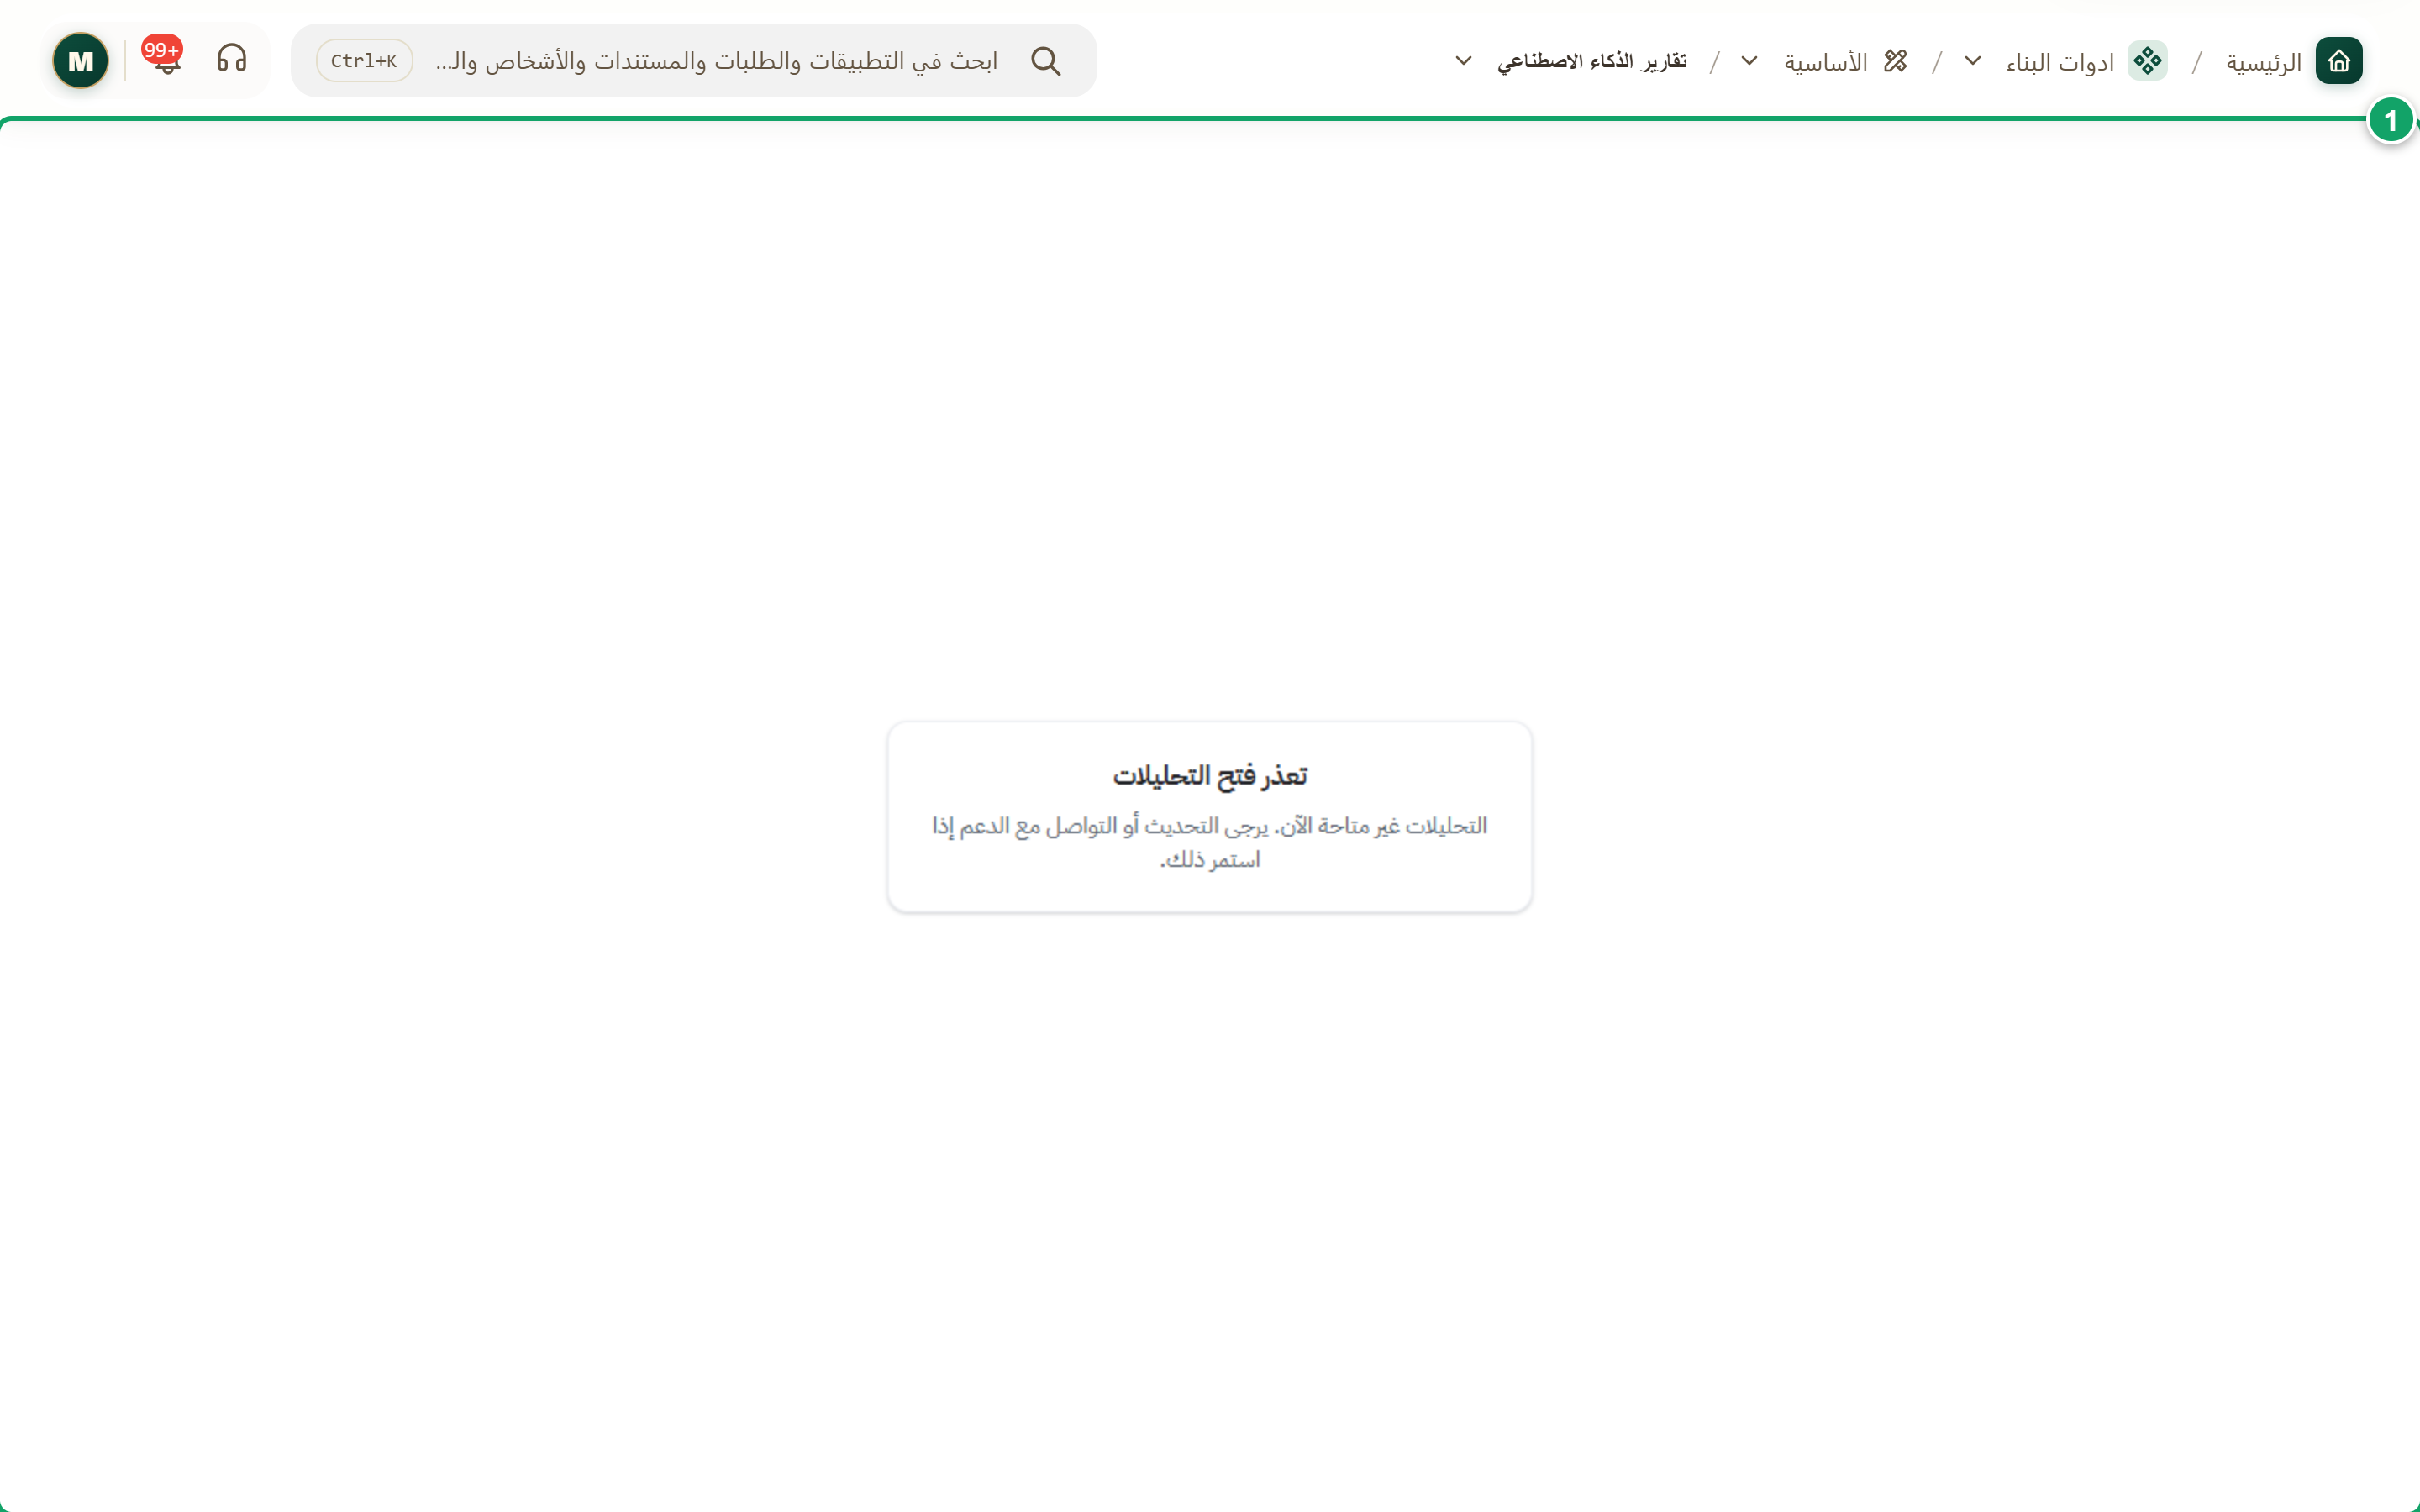
\includegraphics[width=0.95\linewidth,height=0.72\textheight,keepaspectratio]{figures/screens/ch06-ai-reports-ar.png}
\caption{مساحة «تقارير الذكاء الاصطناعي»}
\label{fig:builder-ai-reports-screen}
\shotnote{تُفتح مساحة التحليلات نفسها في وضع المحادثة. ① منطقة المحادثة: تكتب فيها سؤالك وتقرأ التقرير.}
\end{figure}


\begin{table}[H]
\centering
\caption{متى تستخدم التقارير ومتى تستخدم اللوحات؟}
\label{tab:builder-ai-reports-data}
\begin{tabularx}{\linewidth}{R{3.6cm} Y}
\rcHeaderRow
\thh{الحاجة} & \thh{الأنسب}\\
سؤال لمرة واحدة & «تقارير الذكاء الاصطناعي»: اسأل واقرأ الإجابة.\\
متابعة متكررة & «لوحات معلومات الذكاء الاصطناعي» أو «لوحات المعلومات»، لأن اللوحة تُحدَّث وتُراجع دورياً.\\
مشاركة مع الفريق & انشر اللوحة من «الصفحات»؛ فإجابات المحادثة لا تظهر في التنقل.\\
\end{tabularx}
\end{table}

\begin{figure}[H]
\centering
\begin{tikzpicture}[node distance=0.5cm]
\node[stepBox] (a) {\RL{سؤال واضح بفترة محددة}};
\node[stepBox,below=of a] (b) {\RL{قراءة التقرير}};
\node[stepBox,below=of b] (c) {\RL{التحقق من رقم معروف}};
\draw[flowsTo] (a) -- (b);
\draw[flowsTo] (b) -- (c);
\end{tikzpicture}
\rclegend
\caption{طرح سؤال والتحقق من الإجابة}
\label{fig:builder-ai-reports-flow}
\shotnote{ينتهي المخطط بالتحقق، لأن الإجابة مبنية على البيانات التي يستطيع السائل قراءتها وعلى فهم الذكاء الاصطناعي للسؤال. فإذا طابق رقم واحد تعرفه ما في التقرير، زادت ثقتك ببقية الإجابة.}
\end{figure}

\subsection{خطوات العمل والتحقق}
\begin{enumerate}
\item افتح «تقارير الذكاء الاصطناعي»، وانتظر حتى تُحمَّل المحادثة.
\item اكتب سؤالك مع الفترة الزمنية ونوع السجلات المقصود.
\item اقرأ التقرير، وقارن رقماً منه بما تعرفه قبل الاعتماد عليه.
\end{enumerate}

\textbf{تحقق ومعالجة المشكلة:} يجب أن تصل إجابة تشير إلى بيانات مؤسستك. فإذا لم تُفتح الصفحة، فراجع مقعدك وصلاحياتك كما في «لوحات معلومات الذكاء الاصطناعي». وإذا بدت الإجابة ناقصة، فأعد صياغة السؤال بتحديد نوع السجلات والفترة.
